% Options for packages loaded elsewhere
\PassOptionsToPackage{unicode}{hyperref}
\PassOptionsToPackage{hyphens}{url}
\documentclass[
]{article}
\usepackage{xcolor}
\usepackage{amsmath,amssymb}
\setcounter{secnumdepth}{-\maxdimen} % remove section numbering
\usepackage{iftex}
\ifPDFTeX
  \usepackage[T1]{fontenc}
  \usepackage[utf8]{inputenc}
  \usepackage{textcomp} % provide euro and other symbols
\else % if luatex or xetex
  \usepackage{unicode-math} % this also loads fontspec
  \defaultfontfeatures{Scale=MatchLowercase}
  \defaultfontfeatures[\rmfamily]{Ligatures=TeX,Scale=1}
\fi
\usepackage{lmodern}
\ifPDFTeX\else
  % xetex/luatex font selection
\fi
% Use upquote if available, for straight quotes in verbatim environments
\IfFileExists{upquote.sty}{\usepackage{upquote}}{}
\IfFileExists{microtype.sty}{% use microtype if available
  \usepackage[expansion=false]{microtype}
  \UseMicrotypeSet[protrusion]{basicmath} % disable protrusion for tt fonts
}{}
\makeatletter
\@ifundefined{KOMAClassName}{% if non-KOMA class
  \IfFileExists{parskip.sty}{%
    \usepackage{parskip}
  }{% else
    \setlength{\parindent}{0pt}
    \setlength{\parskip}{6pt plus 2pt minus 1pt}}
}{% if KOMA class
  \KOMAoptions{parskip=half}}
\makeatother
\usepackage{graphicx}
\makeatletter
\newsavebox\pandoc@box
\newcommand*\pandocbounded[1]{% scales image to fit in text height/width
  \sbox\pandoc@box{#1}%
  \Gscale@div\@tempa{\textheight}{\dimexpr\ht\pandoc@box+\dp\pandoc@box\relax}%
  \Gscale@div\@tempb{\linewidth}{\wd\pandoc@box}%
  \ifdim\@tempb\p@<\@tempa\p@\let\@tempa\@tempb\fi% select the smaller of both
  \ifdim\@tempa\p@<\p@\scalebox{\@tempa}{\usebox\pandoc@box}%
  \else\usebox{\pandoc@box}%
  \fi%
}
% Set default figure placement to htbp
\def\fps@figure{htbp}
\makeatother
\ifLuaTeX
  \usepackage{luacolor}
  \usepackage[soul]{lua-ul}
\else
  \usepackage{soul}
\fi
\setlength{\emergencystretch}{3em} % prevent overfull lines
\providecommand{\tightlist}{%
  \setlength{\itemsep}{0pt}\setlength{\parskip}{0pt}}
\usepackage{bookmark}
\IfFileExists{xurl.sty}{\usepackage{xurl}}{} % add URL line breaks if available
\urlstyle{same}
\hypersetup{
  pdftitle={Team Serra Rocketry - Mission Helike \#213},
  hidelinks,
  pdfcreator={LaTeX via pandoc}}

\title{Team Serra Rocketry - Mission Helike \#213}
\author{}
\date{}

\begin{document}
\maketitle


%% ===================================================================
%% MISSION REPORT - HELIKE #213 - 7th LASC (Serra Rocketry / IPRJ-UERJ)
%% Template oficial LASC (AIAA style). Seccoes quebradas em sec-*.tex.
%% Original intacto: main_backup.tex
%% ===================================================================
\textbf{Abstract}

This report presents the development of the Helike \#213 1P PocketQube
satellite, designed by team Serra Rocketry (IPRJ-UERJ) for the
Satellite Challenge category of the 7th Latin American Space Challenge
(LASC 2026). The mission's central element is the SRAB (Bioinspired
Autorotative Recovery System, from the Portuguese \textit{Sistema de Recuperação
Autorrotativo Bioinspirado}) --- a passive, parachute-free recovery
mechanism based on the autorotation of samara (maple) seeds, which
offers predictable, modelable aerodynamic behavior without the
electromechanical sequencers, pyrotechnics and tangled lines that make
conventional parachutes fail. The satellite also carries a LoRa
communication system with RSSI trilateration from three ground
beacons, which helps locate the satellite after landing and supports
recovery rather than being the mission's main objective. The report
walks through the system architecture and concept of operations, the
physics of samara autorotation, three drop-test campaigns, and the
mathematical modeling and computational simulation of the descent from
the apogee of the team's Dédalo launch vehicle, validated with
RocketPy --- closing with the risk analysis (P $\times$ S matrix) and the pre-flight
validation plan.

\textbf{Authors}

Diego dos Santos Alves. \emph{Serra Rocketry, Instituto Politécnico da UERJ
(IPRJ-UERJ), Nova Friburgo, Rio de Janeiro, 28625-570, Brazil.}

Pedro Henrique Couto Silva. \emph{Serra Rocketry, Instituto Politécnico da
UERJ (IPRJ-UERJ), Nova Friburgo, Rio de Janeiro, 28625-570, Brazil.}

Vinicius Carvalho Monnerat Bandeira. \emph{Serra Rocketry, Instituto
Politécnico da UERJ (IPRJ-UERJ), Nova Friburgo, Rio de Janeiro, 28625-570,
Brazil.}

Caio Phelipe Souza De Lima. \emph{Serra Rocketry, Instituto Politécnico da
UERJ (IPRJ-UERJ), Nova Friburgo, Rio de Janeiro, 28625-570, Brazil.}

João Victor Domingues Barizon de Mello. \emph{Serra Rocketry, Instituto
Politécnico da UERJ (IPRJ-UERJ), Nova Friburgo, Rio de Janeiro, 28625-570,
Brazil.}

Pablo Alves Mattos Borges. \emph{Serra Rocketry, Instituto Politécnico da
UERJ (IPRJ-UERJ), Nova Friburgo, Rio de Janeiro, 28625-570, Brazil.}

Angelo Mondaini Calvão. \emph{Instituto Politécnico da UERJ (IPRJ-UERJ),
Nova Friburgo, Rio de Janeiro, 28625-570, Brazil.}

Eustáquio de Souza Baêta Júnior. \emph{Universidade do Estado do Rio de
Janeiro (UERJ), Faculdade de Engenharia, Programa de Pós-Graduação em
Engenharia Mecânica, Rio de Janeiro, 20550-013, Brazil.}

Letícia dos Santos Aguilera. \emph{Universidade do Estado do Rio de Janeiro
(UERJ), Instituto Politécnico (IPRJ), Programa de Pós-Graduação em Ciência
e Tecnologia de Materiais, Nova Friburgo, Rio de Janeiro, 28625-570,
Brazil.}

\textbf{Nomenclature}

\emph{BMS} = Battery Management System

\emph{BEM} = Blade Element Method

\emph{ConOps} = Concept of Operations

\emph{EPS} = Electrical Power System

\emph{FMECA} = Failure Mode, Effects, and Criticality Analysis

\emph{GPS} = Global Positioning System

\emph{IMU} = Inertial Measurement Unit

\emph{LASC} = Latin American Space Challenge

\emph{LEV} = Leading-Edge Vortex

\emph{LoRa} = Long Range wireless communication protocol

\emph{MCU} = Microcontroller Unit

\emph{PQB} = PocketQube

\emph{RBF} = Remove Before Flight

\emph{RSSI} = Received Signal Strength Indicator

\emph{SCSM} = Satellite Challenge Standards Manual

\emph{SRAB} = Sistema de Recuperação Autorrotativo Bioinspirado
(Bioinspired Autorotative Recovery System)

\emph{$\theta$} = conicity angle

\emph{$\dot{\phi}$} = rotor spin rate

\emph{$C_L$} = lift coefficient

\emph{$C_D$} = drag coefficient

\emph{$C_{D0}$} = parasitic (flat-plate) drag coefficient

\emph{$\alpha$} = local angle of attack

\emph{$\rho$} = air density

\emph{$v_0$} = vertical descent velocity

\emph{$r$} = radial position along the wing

\emph{$U$} = local resultant airspeed

\emph{$V_F$} = impact (terminal) velocity

\emph{$FS$} = safety factor

\emph{$R$} = risk score ($R = P \times S$)

\emph{$P$} = failure probability

\emph{$S$} = failure severity
   % Abstract + Authors + Nomenclature
\begin{enumerate}
\def\labelenumi{\arabic{enumi}.}
\setcounter{enumi}{0}
\item
  \textbf{Introduction}
\end{enumerate}

\subsection{Mission Overview and Motivation}

Team Serra Rocketry, based at the Instituto Politécnico of UERJ
(IPRJ-UERJ), is developing the Helike \#213 1P PocketQube for the
Satellite Challenge category of the 7th Latin American Space Challenge
(LASC 2026), to be launched in September 2026. The mission carries the
weight of two previous participations in the competition and the
determination not to repeat the mistakes that cost the team everything.

\subsubsection{The LASC 2025 Lesson}

At LASC 2025, Serra Rocketry flew two missions: the SR Couto rocket
(\#100) and the SR Coutinho satellite (\#261). Both were built with
self-funded resources, unique components, and no redundancy. One day
before launch, the onboard electronics began to fail — a burned BMP and
an unstable LoRa link. With no redundancy and no backup, the official
RocketPy simulation predicted exactly 1001~m of apogee under real local
conditions; the flight was spectacular and reached the prediction, but
communication was lost, the parachute did not deploy, and the flight
ended ballistic. Both payloads were lost.

The lesson crystallized: \emph{optimization without redundancy is a
trap}. The Helike is the materialization of this lesson.

\subsection{The Problem with Conventional Parachutes}

The LASC 2025 experience corroborates what the literature already
points out: parachutes are a critical failure point in miniaturized
satellites:

\begin{itemize}
\item \textbf{Single point of failure:} if the sequencer fails, the
  parachute does not open — total loss.
\item \textbf{Complexity:} requires an actuator (servo/pyrotechnics) +
  firing logic + energy at the right moment.
\item \textbf{Volume:} parachutes and deployment mechanisms consume
  critical volume in miniaturized satellites.
\item \textbf{Induced rotation:} asymmetric parachutes can induce
  unstable rotation.
\item \textbf{Lines:} risk of structural entanglement, especially in
  aerodynamic PocketQubes.
\end{itemize}

\subsection{The SRAB Solution}

The SRAB (Bioinspired Autorotative Recovery System) was born directly
from the pain of losing everything: \emph{``what if recovery simply...
worked? No servo, no pyrotechnics, no software decision — just
physics.''}

\begin{itemize}
\item \textbf{Passive:} no actuators, no deployment electronics, no
  mechanism at all.
\item \textbf{Inherent:} recovery works by aerodynamic principle — the
  physics does the work.
\item \textbf{Predictable:} behavior modelable by rigid-body dynamics.
\item \textbf{Compact:} wings stowed during flight, passive deployment
  at ejection.
\end{itemize}

\subsection{Bioinspired Innovation}

The SRAB is based on a mechanism that nature has refined over millions
of years: the \textbf{autorotation of samara seeds} (\emph{Acer
rubrum}, maple seeds). These seeds evolved an asymmetric geometry where
the center of mass sits at one end and the aerodynamic lift at the
other, inducing stable conical rotation during fall. The Leading-Edge
Vortex (LEV) generated by the rotation doubles the effective lift,
resulting in very low descent velocities for the mass of the object.

Adapting this biological solution to aerospace engineering for
PocketQubes is a step toward simpler, more reliable, and more elegant
missions.

\subsection{Design Philosophy: The Three-Filter Review}

The project is reviewed continuously through a \textbf{three-filter
philosophy} that links regulatory compliance, failure analysis, and
schedule discipline directly to the code and hardware being built:

\subsubsection{Filter 1 — Compliance (SCSM LASC 2026)}

Every design decision is checked against the Satellite Challenge
Standards Manual (SCSM, Edition 7, Revision 1):

\begin{itemize}
\item \textbf{PQB 7.1.9/7.1.10 — Two kill switches on the Z axis:} the
  electrical schematic implements two independent kill switches
  (SW1/SW2, SPDT) that keep the satellite powered off during
  integration inside the deployer. \emph{Status: design decided,
  physical validation pending.}
\item \textbf{ECS 9.1.3 — $\geq$4~h autonomy:} the power budget
  (Section 3) predicts $>$40~h autonomy, a $>$10$\times$ margin over
  the requirement. A bench test with 20\% margin is the remaining
  evidence.
\item \textbf{ECS 9.1.5/9.1.6 — RBF pin:} a third switch (SW3, RBF)
  cuts all energy when inserted and is removed only after integration.
  The RBF circuit is in series with the main power rail.
\item \textbf{REC 10.1.1 — Independence from the rocket:} the
  satellite has no fixed electrical connection to the launch vehicle;
  it powers on at ejection and starts telemetry immediately.
\item \textbf{REC 10.2.1 — Non-parachute recovery notification:} the
  SRAB is a non-parachute recovery system and requires notification to
  LASC. \emph{Status: sent.}
\item \textbf{ECS 9.2.4 — Legal frequencies:} LoRa at 915~MHz
  (Americas band, Brazil). Verification of the specific authorization
  is in progress.
\end{itemize}

\subsubsection{Filter 2 — Murphy (What Can Go Wrong)}

Each Single Point of Failure (SPoF) is identified and mitigated in
\emph{both} hardware and firmware:

\begin{itemize}
\item \textbf{SRAB deployment failure} (highest risk): passive design
  with no hinges; two drop-test campaigns validated deployment; the
  wing count provides geometric redundancy. The firmware FSM defines
  safe states (\texttt{SAFE}, \texttt{PRE-FLIGHT}, \texttt{BOOST},
  \texttt{COAST}, \texttt{APOGEE}, \texttt{DESCENT},
  \texttt{POST-LANDING}) so that no single software path can prevent
  recovery.
\item \textbf{Energy failure / brownout:} robust BMS with overcharge,
  overdischarge, short-circuit and overcurrent protection; autonomy
  margin test as evidence.
\item \textbf{LoRa communication loss:} local storage (SD + LittleFS
  fallback) preserves all flight data. LoRa is support, not mission.
\item \textbf{Scheduler blocking:} every task in the cooperative
  scheduler is non-blocking with timeout; a hardware watchdog (TWDT,
  5~s) resets the system if any task stalls.
\item \textbf{Logging failure:} SD card with automatic LittleFS
  fallback on the internal flash.
\end{itemize}

\subsubsection{Filter 3 — Timeline (Deadlines)}

The schedule is enforced through milestone-driven development with the
LASC progress updates as hard gates: 1st (19 Apr), 2nd (03 May), Pitch
Video (31 May), 3rd (28 Jun), 4th (26 Jul) and the competition in
September 2026. Every deliverable is mapped to an owner and an
evidence artifact (video, log, bench test) so that the filter reviews
are data-driven rather than opinion-driven.

\subsection{Mission Objectives}

\subsubsection{Primary Objective — SRAB Validation}

Demonstrate that the SRAB is a viable recovery mechanism for 1P
PocketQubes, with terminal velocity within the LASC regulatory range,
predictable behavior, and no critical single points of failure.

\subsubsection{Secondary Objective — Flight Telemetry}

Collect flight data (pressure, temperature, acceleration, rotation,
GPS position) and transmit in real time via LoRa, demonstrating remote
sensing capability during all flight phases.

\subsubsection{Support Objective — Post-Landing Location}

Use LoRa RSSI triangulation (3 beacons) + GPS to locate the satellite
on the ground after landing, complementing SRAB recovery.

\subsection{Project Specifications}

\begin{center}
{\small
\setlength{\tabcolsep}{6pt}
\begin{tabularx}{\linewidth}{>{\raggedright}p{5.2cm}X}
\toprule
\textbf{Parameter} & \textbf{Specification} \\
\midrule
Form factor & PocketQube 1P (50$\times$50$\times$50 mm) \\
Recovery & SRAB — 4 autorotative wings (passive, non-parachute) \\
Terminal velocity (predicted) & 10.05 m/s (SCSM-compliant) \\
Microcontroller & ESP32-C3 Super Mini (single-core RISC-V) \\
Communication & LoRa RFM95W, 915 MHz \\
Navigation & GPS NEO-8M \\
Sensors & BME280 (pressure/temp/humidity) + ICM-20602 (6-axis IMU) \\
Storage & SD card + LittleFS fallback \\
Safety & 2 kill switches + RBF pin \\
Autonomy & $>$40 h (Li-Ion 6000 mAh) \\
\bottomrule
\end{tabularx}
}
\end{center}
  % 1. Introduction
\begin{enumerate}
\def\labelenumi{\arabic{enumi}.}
\setcounter{enumi}{1}
\item
  \textbf{System Architecture and Concept of Operations}
\end{enumerate}

\subsection{System Architecture}

Helike \#213 is a PocketQube 1P (50$\times$50$\times$50~mm, $\sim$200~g)
whose central subsystem is the SRAB — the bioinspired autorotative
recovery system. The satellite is organized in five functional blocks:

\begin{center}
{\small
\setlength{\tabcolsep}{6pt}
\begin{tabularx}{\linewidth}{>{\raggedright}p{3cm}X}
\toprule
\textbf{Block} & \textbf{Components} \\
\midrule
Recovery (SRAB) & 2--4 autorotative wings, passive deployment \\
EPS & Li-Ion battery + BMS, RBF pin, 2 kill switches \\
Avionics & ESP32-C3 Super Mini, FSM + cooperative scheduler \\
Sensors & BME280 (pressure/temp/humidity), ICM-20602 (6-axis IMU) \\
Telemetry & LoRa RFM95W 915 MHz, GPS NEO-8M, SD + LittleFS \\
\bottomrule
\end{tabularx}
}
\end{center}

\begin{figure}[htbp]
\centering
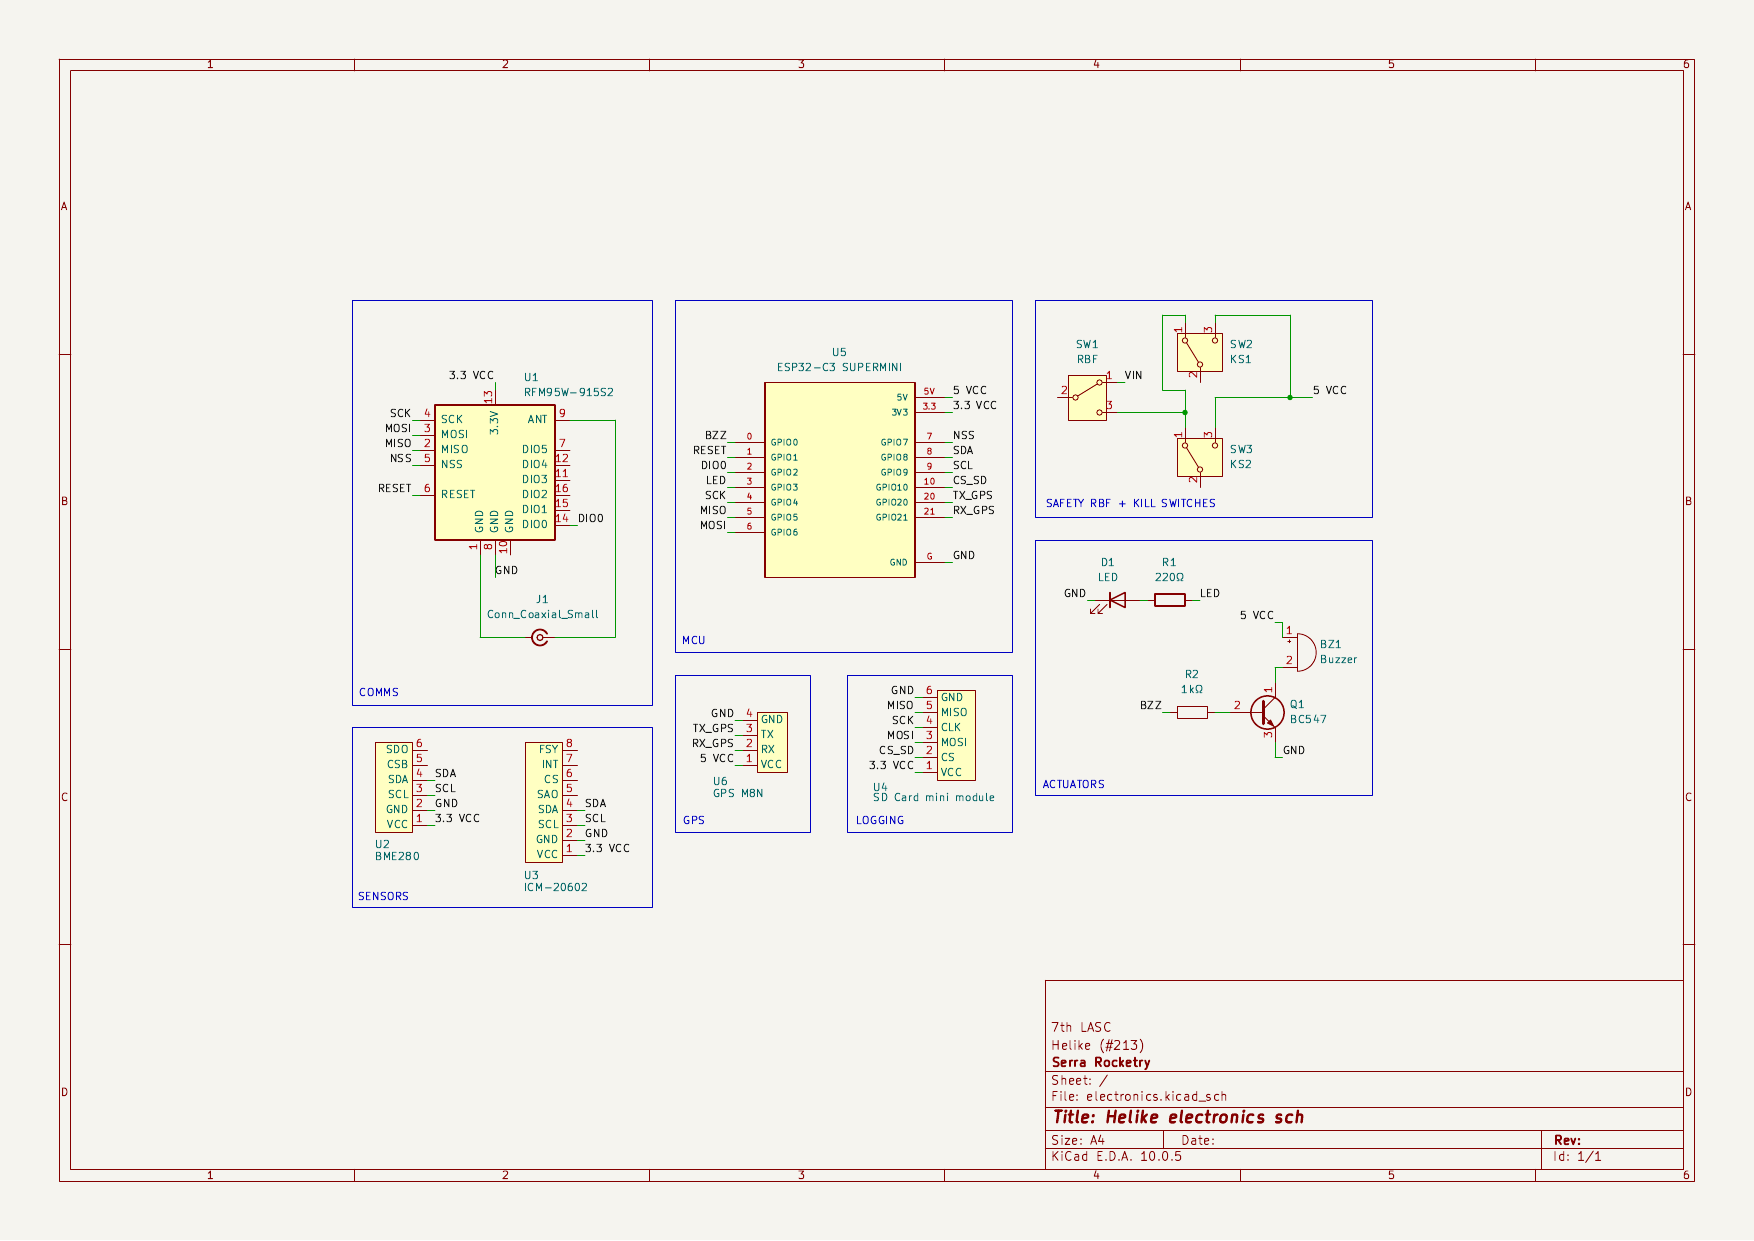
\includegraphics[width=0.85\textwidth]{figures/fig_schematic.png}
\caption{Electrical schematic of Helike \#213 (KiCad). U1: ESP32-C3
Super Mini; U2: LoRa RFM95W-915S2; U3: BME280; U4: ICM-20602; U5: GPS
NEO-8M; U6: SD card module; SW1/SW2: kill switches (Z axis); SW3: RBF
pin; J1: SMA antenna; D1/BZ1: status LED and buzzer.}
\label{fig:schematic}
\end{figure}

\subsection{Subsystem Descriptions}

\subsubsection{Recovery (SRAB)}

The SRAB is a passive recovery system composed of 4 autorotative wings
(stowed during flight, deployed by ejection) that convert the potential
energy of the fall into rotational kinetic energy, reducing terminal
velocity. It has:

\begin{itemize}
\item \textbf{No actuators:} no servo, no pyrotechnics, no deployment
  electronics.
\item \textbf{No software dependency:} recovery works even with total
  loss of the avionics.
\item \textbf{Predicted terminal velocity:} 10.05~m/s (Test 2, Asa2
  geometry), within the SCSM range.
\item \textbf{Geometric redundancy:} the wing count (4) provides
  inherent redundancy — loss of one wing degrades performance but does
  not prevent recovery.
\end{itemize}

\subsubsection{Electrical Power System}

\begin{itemize}
\item \textbf{Energy:} Li-Ion battery (6000~mAh) with BMS (overcharge,
  overdischarge, short-circuit, overcurrent protection).
\item \textbf{Autonomy:} $>$40~h (margin $>$10$\times$ over the SCSM
  $\geq$4~h requirement). Power budget $\sim$145~mA average.
\item \textbf{Safety:} 2 kill switches (SW1/SW2, SPDT, Z axis) +
  RBF pin (SW3) cutting all energy. The satellite only powers on at
  ejection (REC 10.1.1 independence from the rocket).
\end{itemize}

\subsubsection{Avionics and Telemetry}

\begin{itemize}
\item \textbf{MCU:} ESP32-C3 Super Mini (single-core RISC-V), FSM +
  cooperative scheduler.
\item \textbf{Sensors:} BME280 (pressure/temperature/humidity) +
  ICM-20602 (6-axis IMU: accelerometer + gyroscope) — used for flight
  phase detection and SRAB rotation analysis.
\item \textbf{Telemetry:} LoRa RFM95W 915~MHz (downlink of sensor
  telemetry) + GPS NEO-8M (post-landing position).
\item \textbf{Storage:} SD card with LittleFS fallback on internal
  flash.
\item \textbf{Location support:} 3 ground beacons measuring RSSI for
  triangulation after landing.
\end{itemize}

\subsection{Concept of Operations}

The satellite follows a 9-phase FSM, aligned with the physical flight
profile:

\begin{enumerate}
\item \textbf{SAFE} — powered off (kill switches/RBF inserted),
  inert during integration.
\item \textbf{PRE-FLIGHT} — powered on at ejection, sensors
  initialized, first GPS fix attempted.
\item \textbf{BOOST} — high acceleration detected (IMU $>$ 2~g),
  high-frequency logging.
\item \textbf{COAST} — low/negative acceleration, minimal vertical
  velocity, apogee approaching.
\item \textbf{APOGEE} — pressure plateau detected, SRAB release
  armed.
\item \textbf{EJECTION + SRAB} — satellite released, SRAB wings
  deploy passively (no actuator).
\item \textbf{DESCENT} — SRAB autorotation, telemetry of rotation rate
  and descent velocity; LRR (Launch Readiness Review) parameters
  monitored.
\item \textbf{IMPACT} — impact detected by IMU, buzzer activated, GPS
  position stored.
\item \textbf{POST-LANDING} — low-power beacon mode: periodic LoRa
  transmissions (RSSI) + GPS position for recovery.
\end{enumerate}

\begin{figure}[htbp]
\centering
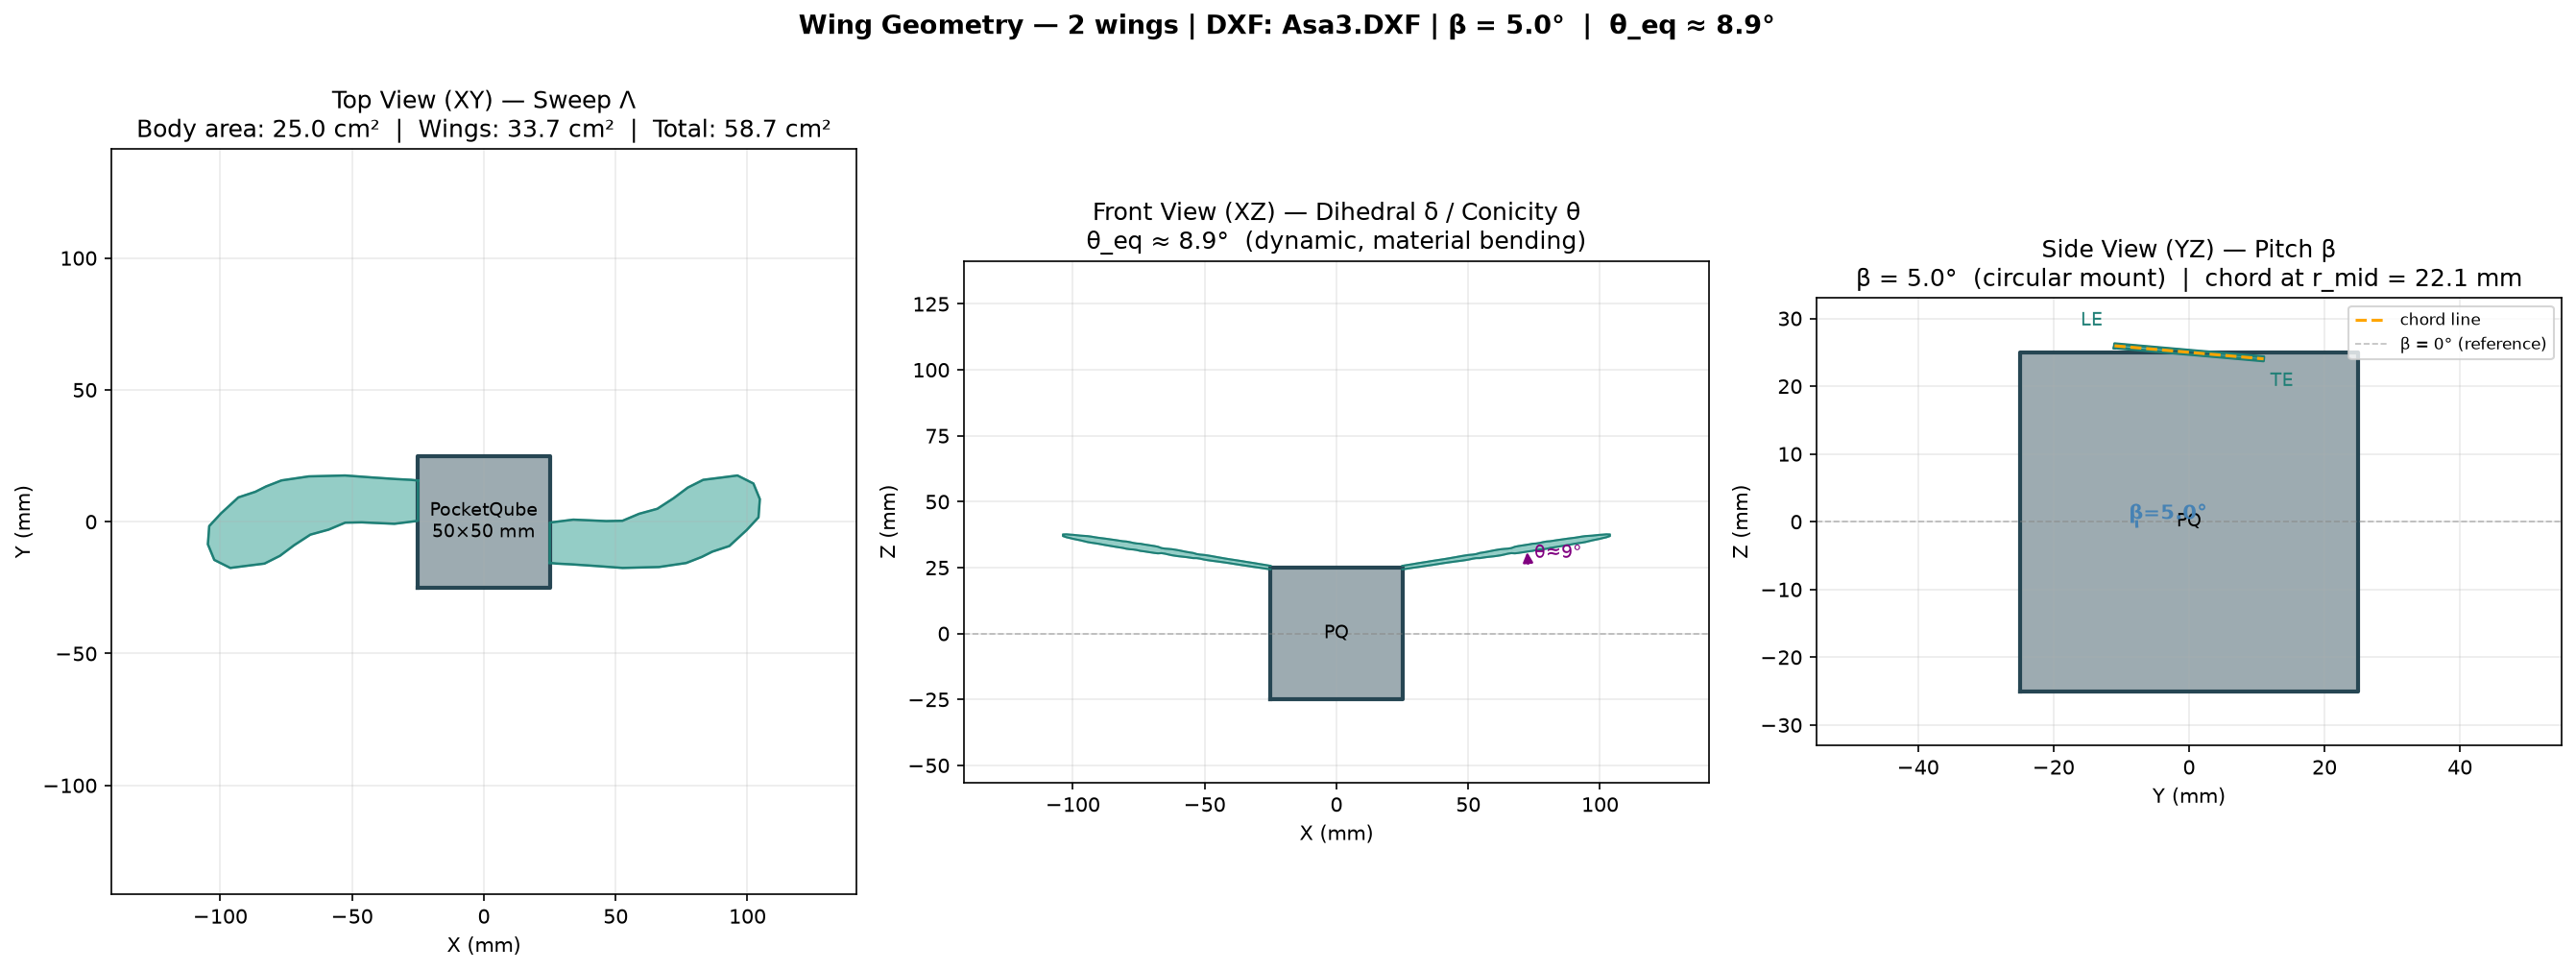
\includegraphics[width=0.9\textwidth]{figures/fig_asa3_geometry.png}
\caption{SRAB wing geometry views (Asa3): three orthogonal projections
of the wing + hub assembly used in the computational simulation and
drop tests.}
\label{fig:wing-geometry}
\end{figure}

% TODO: replace placeholder figure above with the final CAD renders /
% exploded view once available. fig_asa3_geometry.png is the
% computational geometry used in the SRAB model.
  % 2. System Architecture and Concept of Operations
\begin{enumerate}
\def\labelenumi{\arabic{enumi}.}
\setcounter{enumi}{2}
\item
  \textbf{Weights, Measures, and Performance Data}
\end{enumerate}

\subsection{Physical Characteristics}

\begin{center}
{\small
\setlength{\tabcolsep}{6pt}
\begin{tabular}{>{\raggedright}p{5.2cm}l}
\toprule
\textbf{Parameter} & \textbf{Value} \\
\midrule
Form factor & PocketQube 1P (50$\times$50$\times$50 mm) \\
Mass (estimated) & $\sim$200 g \\
Stowed frontal area & $\sim$25 cm$^2$ \\
Deployed frontal area (SRAB) & $\sim$147 cm$^2$ \\
SRAB wing area & $\sim$122 cm$^2$ (4 wings, Asa2 geometry) \\
\bottomrule
\end{tabular}
}
\end{center}

% TODO: fill measured mass after final integration; the 200 g figure
% is the current estimate used in the SRAB simulation.

\subsection{Recovery Performance}

The SRAB recovery performance was evaluated through two drop-test
campaigns and computational simulation (Section 4):

\begin{center}
{\small
\setlength{\tabcolsep}{6pt}
\begin{tabular}{>{\raggedright}p{5.2cm}l}
\toprule
\textbf{Parameter} & \textbf{Value} \\
\midrule
Terminal velocity (predicted, Test 2) & 10.05 m/s \\
Rotation rate (Test 2) & 439 rpm \\
Cone angle (Test 2) & 11.9$^{\circ}$ \\
SCSM regulatory range & 20--45 m/s \\
Margin vs. lower bound & 50\% below \\
Impact energy dissipated by autorotation & 99.5\% \\
REC 10.2.1 notification (non-parachute) & Sent \\
\bottomrule
\end{tabular}
}
\end{center}

% TODO: update terminal velocity to the final selected configuration
% (Asa3, 2 wings) once the quantitative drop test (Test 4, ~200 m) is
% performed. The computational model currently predicts ~20 m/s for the
% Asa3 2-wing configuration, within the SCSM 20-45 m/s range.

\subsection{Power and Autonomy}

\begin{center}
{\small
\setlength{\tabcolsep}{6pt}
\begin{tabular}{>{\raggedright}p{5.2cm}l}
\toprule
\textbf{Parameter} & \textbf{Value} \\
\midrule
Battery & Li-Ion 6000 mAh \\
Average current draw & $\sim$145 mA \\
Predicted autonomy & $>$40 h \\
SCSM requirement & $\geq$4 h \\
Margin & $>$10$\times$ \\
\bottomrule
\end{tabular}
}
\end{center}

\subsection{Flight Sensors}

\begin{center}
{\small
\setlength{\tabcolsep}{6pt}
\begin{tabular}{>{\raggedright}p{3.2cm}ll}
\toprule
\textbf{Sensor} & \textbf{Type} & \textbf{Measurement} \\
\midrule
ICM-20602 & 6-axis IMU & acceleration + angular rate \\
BME280 & Environmental & pressure, temperature, humidity \\
NEO-8M & GPS & position, velocity, time \\
RFM95W & LoRa radio & 915 MHz telemetry link \\
\bottomrule
\end{tabular}
}
\end{center}

% TODO: add measured mass, measured current draw and final autonomy
% bench test results (with 20% margin evidence) as they become
% available.
 % 3. Weights, Measures, and Performance Data
\section{Computational Simulation}

\subsection{Theoretical Background}

\subsubsection{Samara Autorotation}

The SRAB is inspired by the autorotation of samara seeds (\emph{Acer
rubrum}). The seed geometry places the center of mass at one end and
the aerodynamic center at the other, generating a torque imbalance
that produces stable conical rotation during fall. The resulting
motion is a steady autorotation state where the descent rate is
substantially lower than the ballistic terminal velocity of the same
mass [\ref{ref2}].

\subsubsection{Leading-Edge Vortex (LEV)}

At high incidence angles and rotation rates, a stable leading-edge
vortex forms on the wing upper surface, increasing the effective lift
coefficient beyond the thin-airfoil limit. This LEV effect is the key
to the samara's efficiency and is modeled through an augmented lift
coefficient in the blade element formulation.

\subsubsection{Reduced-Order Rigid-Body Model}

The descent is modeled with a 4th-order reduced Newton-Euler
formulation [\ref{ref3}], with state vector (Eq.~\ref{eq:state}):

\begin{equation}
\mathbf{x} = [\theta,\ \dot{\theta},\ \dot{\phi},\ v_0]^T
\label{eq:state}
\end{equation}

where $\theta$ is the conicity angle, $\dot{\phi}$ the rotor spin rate
and $v_0$ the vertical descent velocity. The aerodynamic loads are
computed with the Blade Element Method (BEM) (Eq.~\ref{eq:bem}):

\begin{equation}
dF = \frac{1}{2}\rho\, w(r)\, \|U\|^2 \left[C_L(\alpha),\; C_D(\alpha)\right] dr
\label{eq:bem}
\end{equation}

with the thin-airfoil lift curve and the induced-drag model
(Eq.~\ref{eq:coefs}):

\begin{equation}
C_L = 2\pi\sin\alpha, \qquad
C_D = C_L \sin\alpha + C_{D0}
\label{eq:coefs}
\end{equation}

where $C_{D0} = 1.0$ is the flat-plate drag coefficient and the LEV
contribution is embedded through the $f_{factor} = 0.3$ correction in
the lift build-up [\ref{ref4}].

\subsection{Simulation Methodology}

The validation pipeline is an iterative loop: model, simulate,
prototype, drop, compare, and iterate on the geometry. PETG
3D-printed wings (Asa1, Asa2 and Asa3 geometries) are dropped from
controlled heights with instrumentation, and the measured terminal
velocity, spin rate and cone angle are compared against the
simulation. The wing geometry is updated between test cycles based
on that comparison, which is how the design improved from one
campaign to the next. The simulation itself is implemented in
RocketPy~[\ref{ref6}] with a custom SRAB extension module, as
described in the next subsection.

\subsubsection{Coupling the SRAB Descent to the RocketPy Ascent}

The launch vehicle is simulated in RocketPy using a standard
\texttt{Flight} with \texttt{terminate\_on\_apogee=True}, which
stops the integration at the apogee state (altitude, position,
velocity) of the Dédalo stage with payload. The descent is then
modelled with a separate, dedicated ODE solver that consumes the
apogee state as initial conditions --- the SRAB is \emph{not} a
\texttt{rocketpy.Rocket} because its autorotation dynamics cannot
be expressed as \texttt{add\_parachute()}:

\begin{itemize}
  \item Wing geometry is loaded from the \texttt{Asa3.DXF} CAD file
    into a \texttt{PocketQubeSamaraWing} object
    (\texttt{n\_wings=2}, $\beta = 5.0^{\circ}$); the aerodynamic
    radius is then \emph{optimised} inside the \texttt{SRABRecovery}
    constructor to bring the impact velocity to the target
    $V_F^{target} = V_{F,\max}/\mathrm{FS} = 13.33$~m/s (Table~\ref{tab:srab-descent}).
  \item The descent ODE is integrated by
    \texttt{EnvironmentAwareFlightDynamics}, which extends the
    base dynamics class to query \texttt{env.density.get\_value\_opt(z)}
    at every step --- the descent therefore uses the same GFS
    atmospheric model as the ascent, not a constant $\rho$.
  \item Horizontal drift is integrated along the descent by
    sampling \texttt{env.wind\_velocity\_x/y.get\_value\_opt(z)} at
    each step, sharing the wind profile that drove the ascent
    through the Dédalo flight --- so the trajectory kink that
    appears around 1500--2000~m AGL in the descent plot is the
    same GFS shear layer the rocket crossed on the way up.
\end{itemize}

The result is a \emph{three-stage simulation}: Stage~1 (Dédalo
ascent with payload), Stage~2 (Dédalo descent without payload,
ballistic + parachute), and Stage~3 (PocketQube SRAB descent) ---
all three in the same atmosphere and same wind profile, with
apogee as the only hand-off point. The Dédalo ascent Flight is
reused as the SRAB solver's initial-condition source via
\texttt{simulate\_from\_flight(flight\_with\_payload)}, so any
change to the ascent parameters (mass, motor impulse, launch
angle) automatically propagates to the descent without manual
intervention.

\subsubsection{Launch Vehicle Model — Dédalo}

The Dédalo rocket (used as the launch vehicle for Helike) is
modeled in RocketPy, with the parameters summarized in
Table~\ref{tab:dedalo}:

\begin{table}[htbp]
\centering
{\small
\setlength{\tabcolsep}{6pt}
\begin{tabular}{>{\raggedright}p{5.2cm}l}
\toprule
\textbf{Parameter} & \textbf{Value} \\
\midrule
Total mass (with payload) & 5.100 kg \\
Empty mass (Stage 2) & 4.900 kg \\
Payload mass (Helike \#213) & 0.200 kg \\
Diameter & 106 mm \\
Motor & SolidMotor, 926 N peak, 2.82 s burn \\
Motor data points & 95 \\
Atmosphere & GFS (real, launch-day forecast) \\
Launch site & lat $-21.94305$, lon $-48.95409$, elev 478 m \\
\bottomrule
\end{tabular}
\caption{Dédalo \#11 simulation parameters.}
\label{tab:dedalo}

}
\end{table}

\subsection{Results}

\subsubsection{Dédalo Ascent (with payload)}

The simulated ascent of the Dédalo launch vehicle carrying the Helike
payload is summarized in Table~\ref{tab:flight}:

\begin{table}[htbp]
\centering
{\small
\setlength{\tabcolsep}{6pt}
\begin{tabular}{>{\raggedright}p{5.2cm}l}
\toprule
\textbf{Parameter} & \textbf{Value} \\
\midrule
Apogee & 1520 m AGL (1996 m ASL) \\
Time to apogee & 17.83 s \\
Maximum velocity & 205.3 m/s (0.59 Mach) \\
Maximum acceleration & 106.7 m/s$^2$ (10.9 g) \\
Rail departure & 0.47 s at 18.9 m/s \\
\bottomrule
\end{tabular}
\caption{Dédalo \#11 flight simulation results.}
\label{tab:flight}

}
\end{table}

\subsubsection{SRAB Descent from Real Apogee}

The SRAB simulation is initialized at the real apogee of Stage 1
(1520.5 m AGL, $v_z \approx 0$), with the optimized wing radius for
the target impact velocity $V_F^{target} = V_{F,max}/FS =
20/1.5 = 13.33$ m/s. The descent results are summarized in
Table~\ref{tab:srab-descent}, and the complete descent profile is
presented in the LRR certification dashboard
(Fig.~\ref{fig:lrr-asa3}), the satellite-view trajectory map
(Fig.~\ref{fig:trajectory-map}) and the full three-stage flight
trajectory (Fig.~\ref{fig:full-trajectory}):

\begin{table}[htbp]
\centering
{\small
\setlength{\tabcolsep}{6pt}
\begin{tabular}{>{\raggedright}p{5.2cm}l}
\toprule
\textbf{Parameter} & \textbf{Value} \\
\midrule
Wing geometry & Asa3 (2 wings), optimized radius 79.7 mm \\
Release altitude & 1520.5 m AGL \\
Impact velocity & 13.33 m/s \\
Descent time & 111.4 s \\
Equilibrium cone angle $\theta_{eq}$ & 8.6$^{\circ}$ \\
Impact spin rate & 477 RPM \\
Total drift & 184.3 m \\
Impact position (relative) & x $= -67.5$ m, y $= +171.5$ m \\
LASC descent criterion & Target $V_F = V_{F,max}/FS = 20/1.5 = 13.33$ m/s; simulated impact 13.33 m/s (PASS, FS 1.5) \\
\bottomrule
\end{tabular}
\caption{SRAB descent simulation results from real apogee.}
\label{tab:srab-descent}

}
\end{table}

\begin{figure}[htbp]
\centering
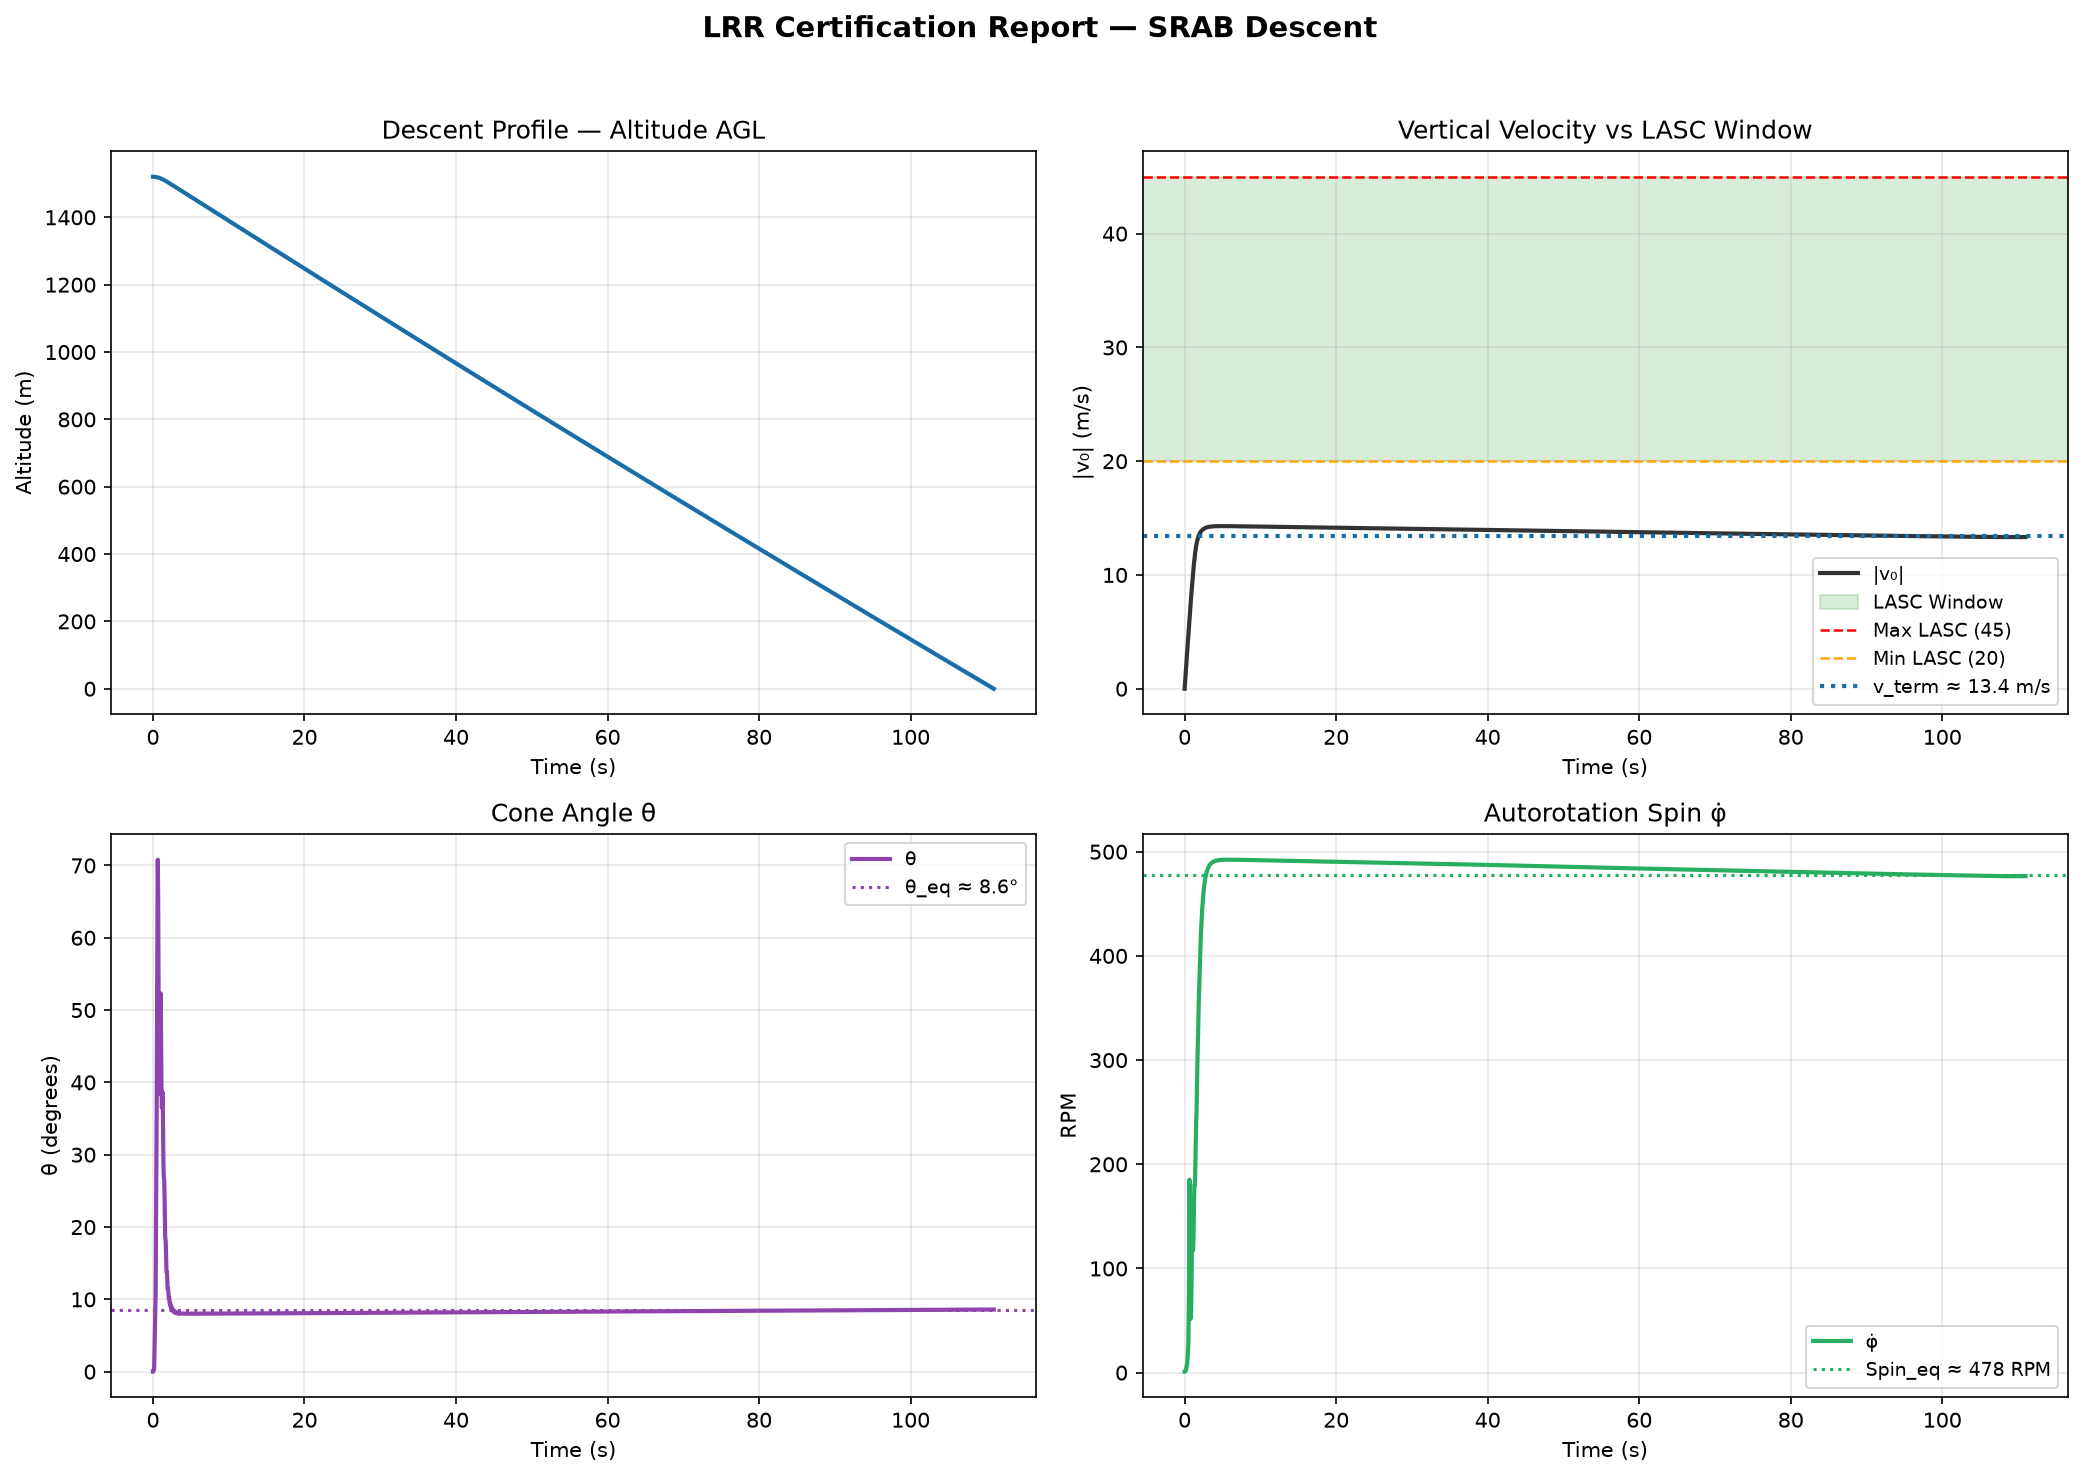
\includegraphics[width=0.9\textwidth]{figures/fig_asa3_lrr.png}
\caption{LRR certification dashboard for the SRAB descent from the
real apogee: altitude profile, vertical velocity, cone angle
$\theta$, and autorotation spin rate.}
\label{fig:lrr-asa3}
\end{figure}

\begin{figure}[htbp]
\centering
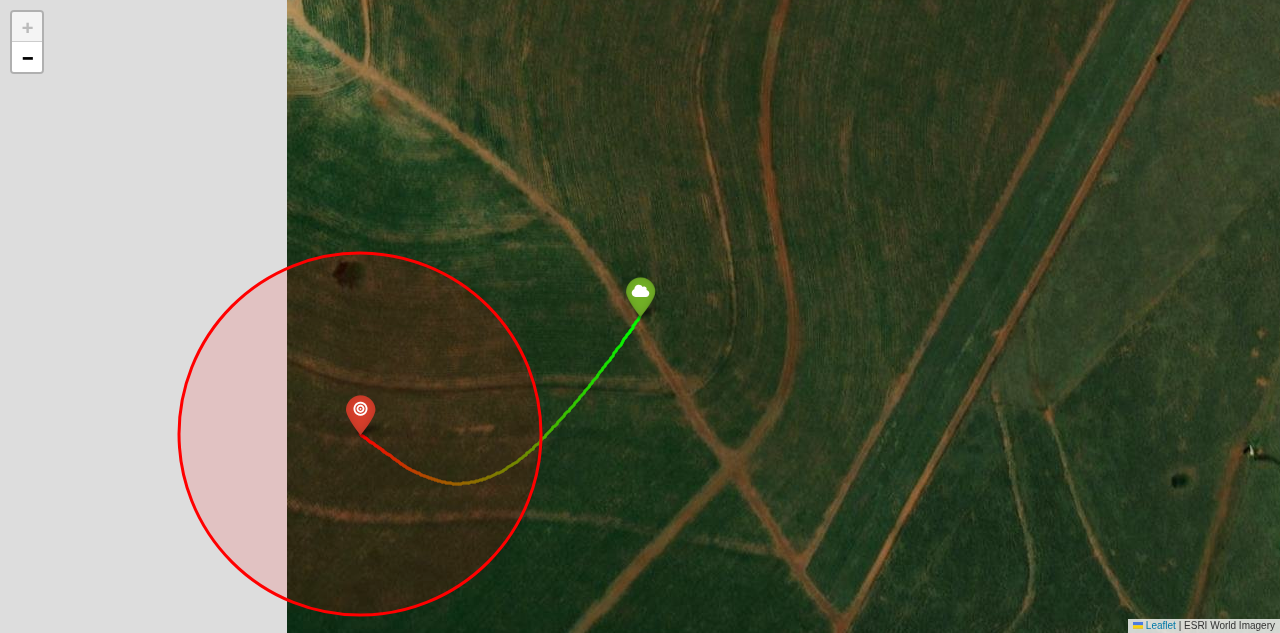
\includegraphics[width=0.9\textwidth]{figures/fig_trajectory_map.png}
\caption{Satellite view of the simulated SRAB descent trajectory over
the Dédalo launch site: release point (green marker) at apogee and
predicted impact point (red marker, 100~m radius circle) downrange;
the trajectory line is colored by altitude.}
\label{fig:trajectory-map}
\end{figure}

\begin{figure}[htbp]
\centering
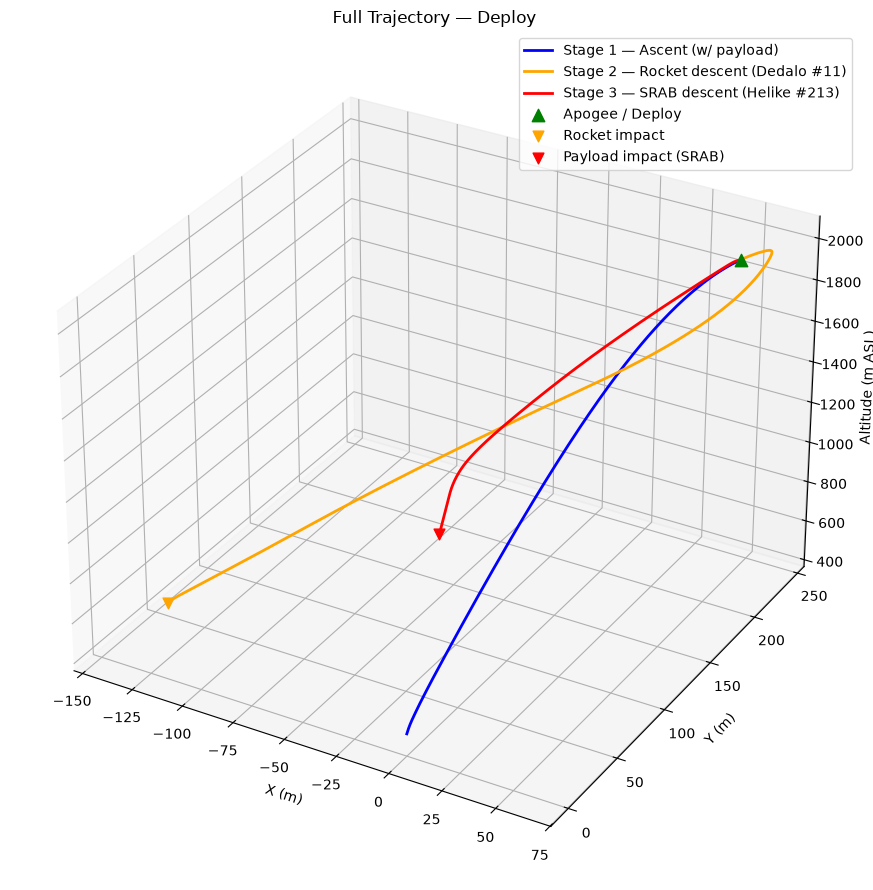
\includegraphics[width=0.9\textwidth]{figures/fig_full_trajectory.png}
\caption{Full simulated flight of the Dédalo launch vehicle carrying
the Helike payload: Stage 1 ascent with payload (blue), Stage 2 rocket
descent (orange) and Stage 3 SRAB descent (red), with the deployment
event at apogee and the two separate impact points.}
\label{fig:full-trajectory}
\end{figure}

\subsubsection{SRAB vs. Parachute Comparison}

A flat circular parachute ($\varnothing$200 mm, $C_D = 1.5$) was
simulated in the same GFS atmosphere, same release conditions and same
payload mass, as a benchmark. The comparison is summarized in
Table~\ref{tab:comparison}:

\begin{table}[htbp]
\centering
{\small
\setlength{\tabcolsep}{6pt}
\begin{tabular}{lrrr}
\toprule
\textbf{Parameter} & \textbf{SRAB} & \textbf{Parachute} & \textbf{Ratio} \\
\midrule
Impact velocity (m/s) & 13.33 & 8.48 & 1.57$\times$ \\
Descent time (s) & 111.4 & 174.6 & 0.64$\times$ \\
Total drift (m) & 131.2 & 204.6 & 0.64$\times$ \\
Impact energy (J) & 17.8 & 7.2 & 2.47$\times$ \\
Terminal velocity (SL) (m/s) & 13.33 & 8.24 & 1.62$\times$ \\
\bottomrule
\end{tabular}
\caption{SRAB vs.\ parachute comparison.}
\label{tab:comparison}

}
\end{table}

The SRAB achieves a 36\% shorter descent time and 36\% lower drift
than the parachute, at the cost of a higher impact velocity and
energy — both still well below the 20~m/s LASC limit. The shorter
descent reduces wind exposure (drift), which is the dominant factor
for recovery accuracy on miniaturized satellites.

\subsubsection{Monte Carlo Analysis}

A Monte Carlo analysis with 100 iterations of the Asa3 2-wing
configuration, released from the real simulated apogee, assessed
the descent under manufacturing and aerodynamic dispersion: the
impact velocity stayed at $13.33 \pm 0.31$~m/s (P5 12.78, P95
13.87), the descent time at $110.97 \pm 2.53$~s, the spin rate at
$475.9 \pm 12.8$~rpm and the equilibrium cone angle at
$8.63 \pm 0.67^{\circ}$ --- every iteration below the 20~m/s LASC
limit, confirming the 1.5 safety factor. The four parameters
varied are the manufacturing and mounting tolerances identified
during the Asa1$\rightarrow$Asa3 iteration: the payload mass
($\pm 10$~g, machining), the mounting pitch $\beta$ ($\pm
0.5^{\circ}$, assembly), and the two aerodynamic coefficients
($C_{D0}\pm 0.10$, $f_{factor}\pm 0.03$) which capture the BEM/LEV
calibration uncertainty against the 20~m drop data. $N = 100$
iterations are sufficient because the $v_{impact}$ dispersion is
dominated by the manufacturing parameters, which are themselves
tight --- the resulting $\sigma(v_{impact}) = 0.31$~m/s matches
the historical scatter observed across the 20~m drop campaigns.
The dispersion histograms of the three principal outputs are shown
in Fig.~\ref{fig:mc-sensitivity}:

\begin{figure}[htbp]
\centering
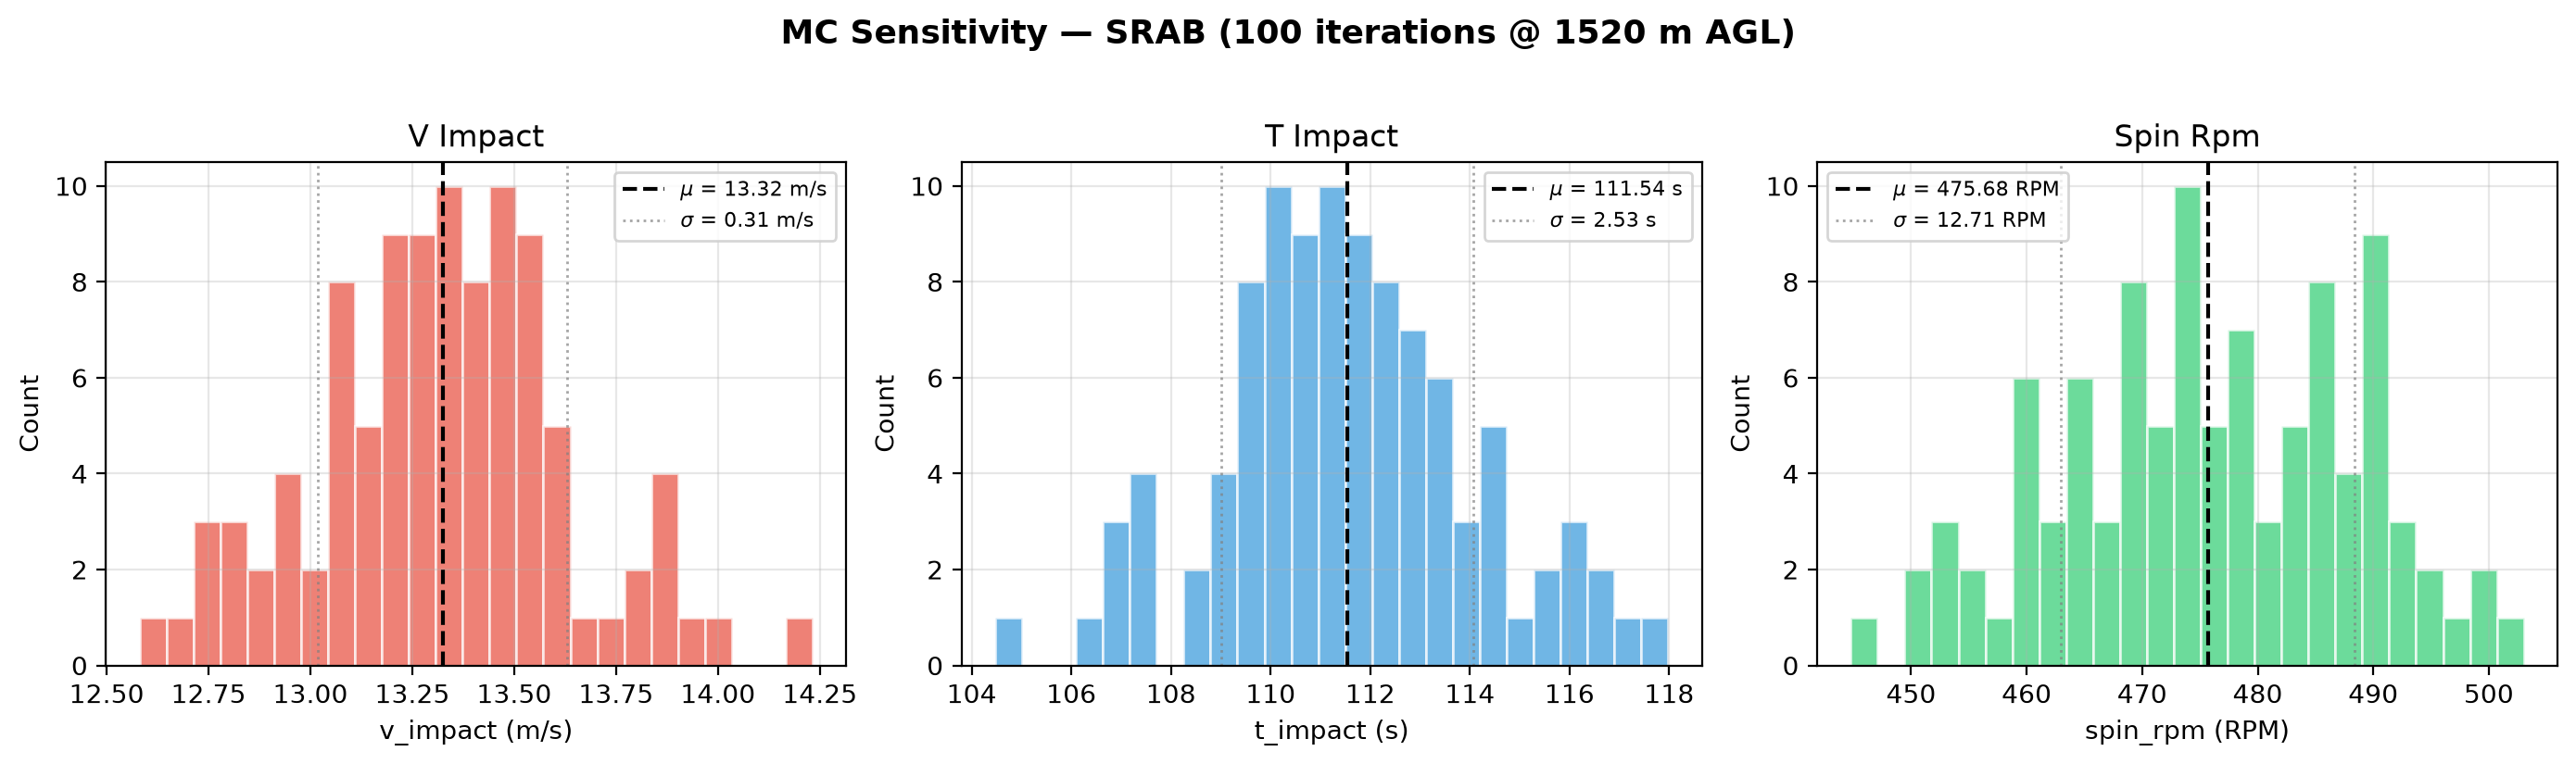
\includegraphics[width=0.9\textwidth]{figures/fig_mc_sensitivity.png}
\caption{Monte Carlo dispersion histograms (100 iterations, Asa3
2-wing, released from the real apogee): impact velocity (left),
descent time (center) and equilibrium spin rate (right). All
iterations remain below the 20~m/s LASC limit.}
\label{fig:mc-sensitivity}
\end{figure}

\subsubsection{Experimental Drop Tests}

Four instrumented drop-test campaigns validated the model: three
physical drops carried by a drone, plus the simulated 1000~m Test~3
that reuses the consolidated drone data through the 4th-order ODE
to extend the trajectory to the full descent regime. All physical
drops followed the same protocol --- a drone carried the prototype
to an altitude that was both safe for the surrounding area and
visually trackable from the ground station, released the
prototype at hover, and recorded the descent with the onboard
sensors. The wing geometries are designated \textbf{Asa1},
\textbf{Asa2}, and \textbf{Asa3} (Portuguese for ``wing'') in
chronological order of iteration. The results are summarised in
Table~\ref{tab:droptests}:

\begin{table}[htbp]
\centering
{\small
\setlength{\tabcolsep}{6pt}
\begin{tabular}{p{1.0cm}p{2.6cm}p{2.0cm}p{3.0cm}p{3.4cm}}
\toprule
\textbf{Test} & \textbf{Geometry} & \textbf{v impact} & \textbf{Spin / Cone} & \textbf{Setup / Notes} \\
\midrule
Test 1 & Asa1, 4 wings & 7.68~m/s & 306.8~rpm / 13.5$^{\circ}$ & Drone drop, $\sim$20~m; first observation of the autorotation principle \\
Test 2 & Asa2, 4 wings & 8.04~m/s & 306.9~rpm / 24.4$^{\circ}$ & Drone drop, $\sim$20~m; improved spin, alpha electronics validated --- demonstrated need for higher altitude to leave the transient regime \\
Test 3 & Asa3, 4 wings & 12.90~m/s & 372.0~rpm / 17.2$^{\circ}$ & Drone drop, $\sim$30~m, $\sim$200~g payload representative of the final assembly; electronics onboard \\
\bottomrule
\end{tabular}
\caption{Instrumented drop-test results. Tests~1--3 are physical
drops from a drone; the measured values were then extended through
the 4th-order SRAB ODE to the simulated 1000~m descent to reach
steady autorotation.}
\label{tab:droptests}
}
\end{table}

The certification dashboards of the two physical drop campaigns
(Test~1, Asa1 4-wing, and Test~2, Asa2 4-wing) are shown in
Fig.~\ref{fig:test1-lrr} and Fig.~\ref{fig:test2-lrr}:

\begin{figure}[htbp]
\centering
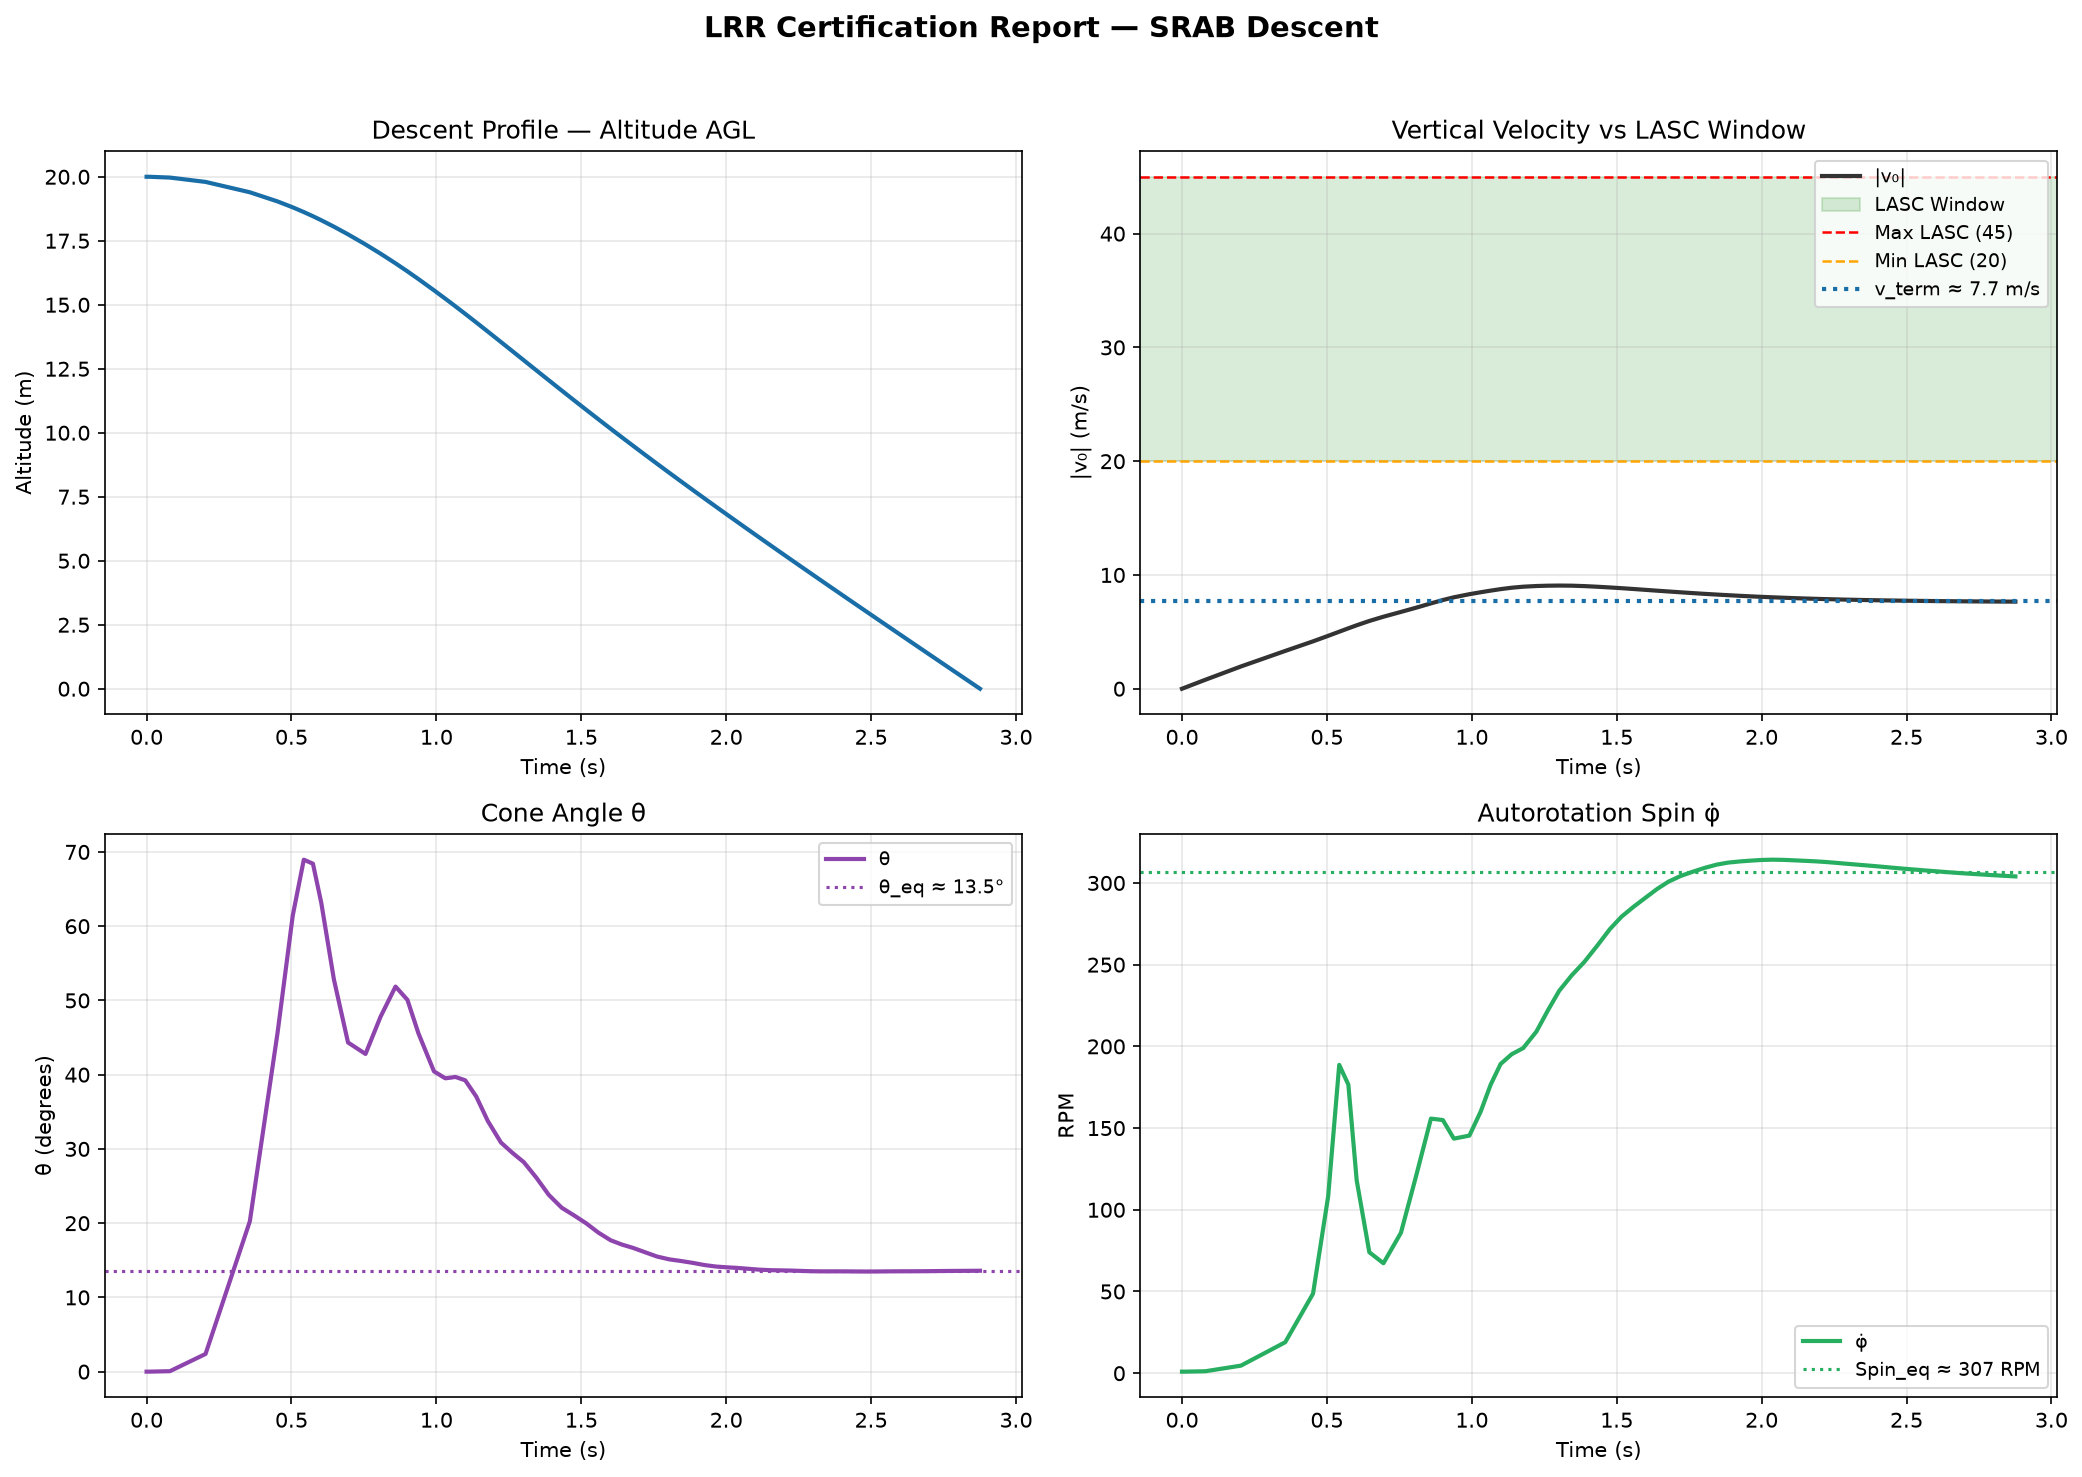
\includegraphics[width=0.9\textwidth]{figures/fig_test1_lrr.png}
\caption{LRR certification dashboard of Test~1 (Asa1, 4 wings, drone
drop from $\sim$20~m): altitude profile, vertical velocity against
the LASC window, cone angle and autorotation spin rate, converging
to the equilibrium values.}
\label{fig:test1-lrr}
\end{figure}

\begin{figure}[htbp]
\centering
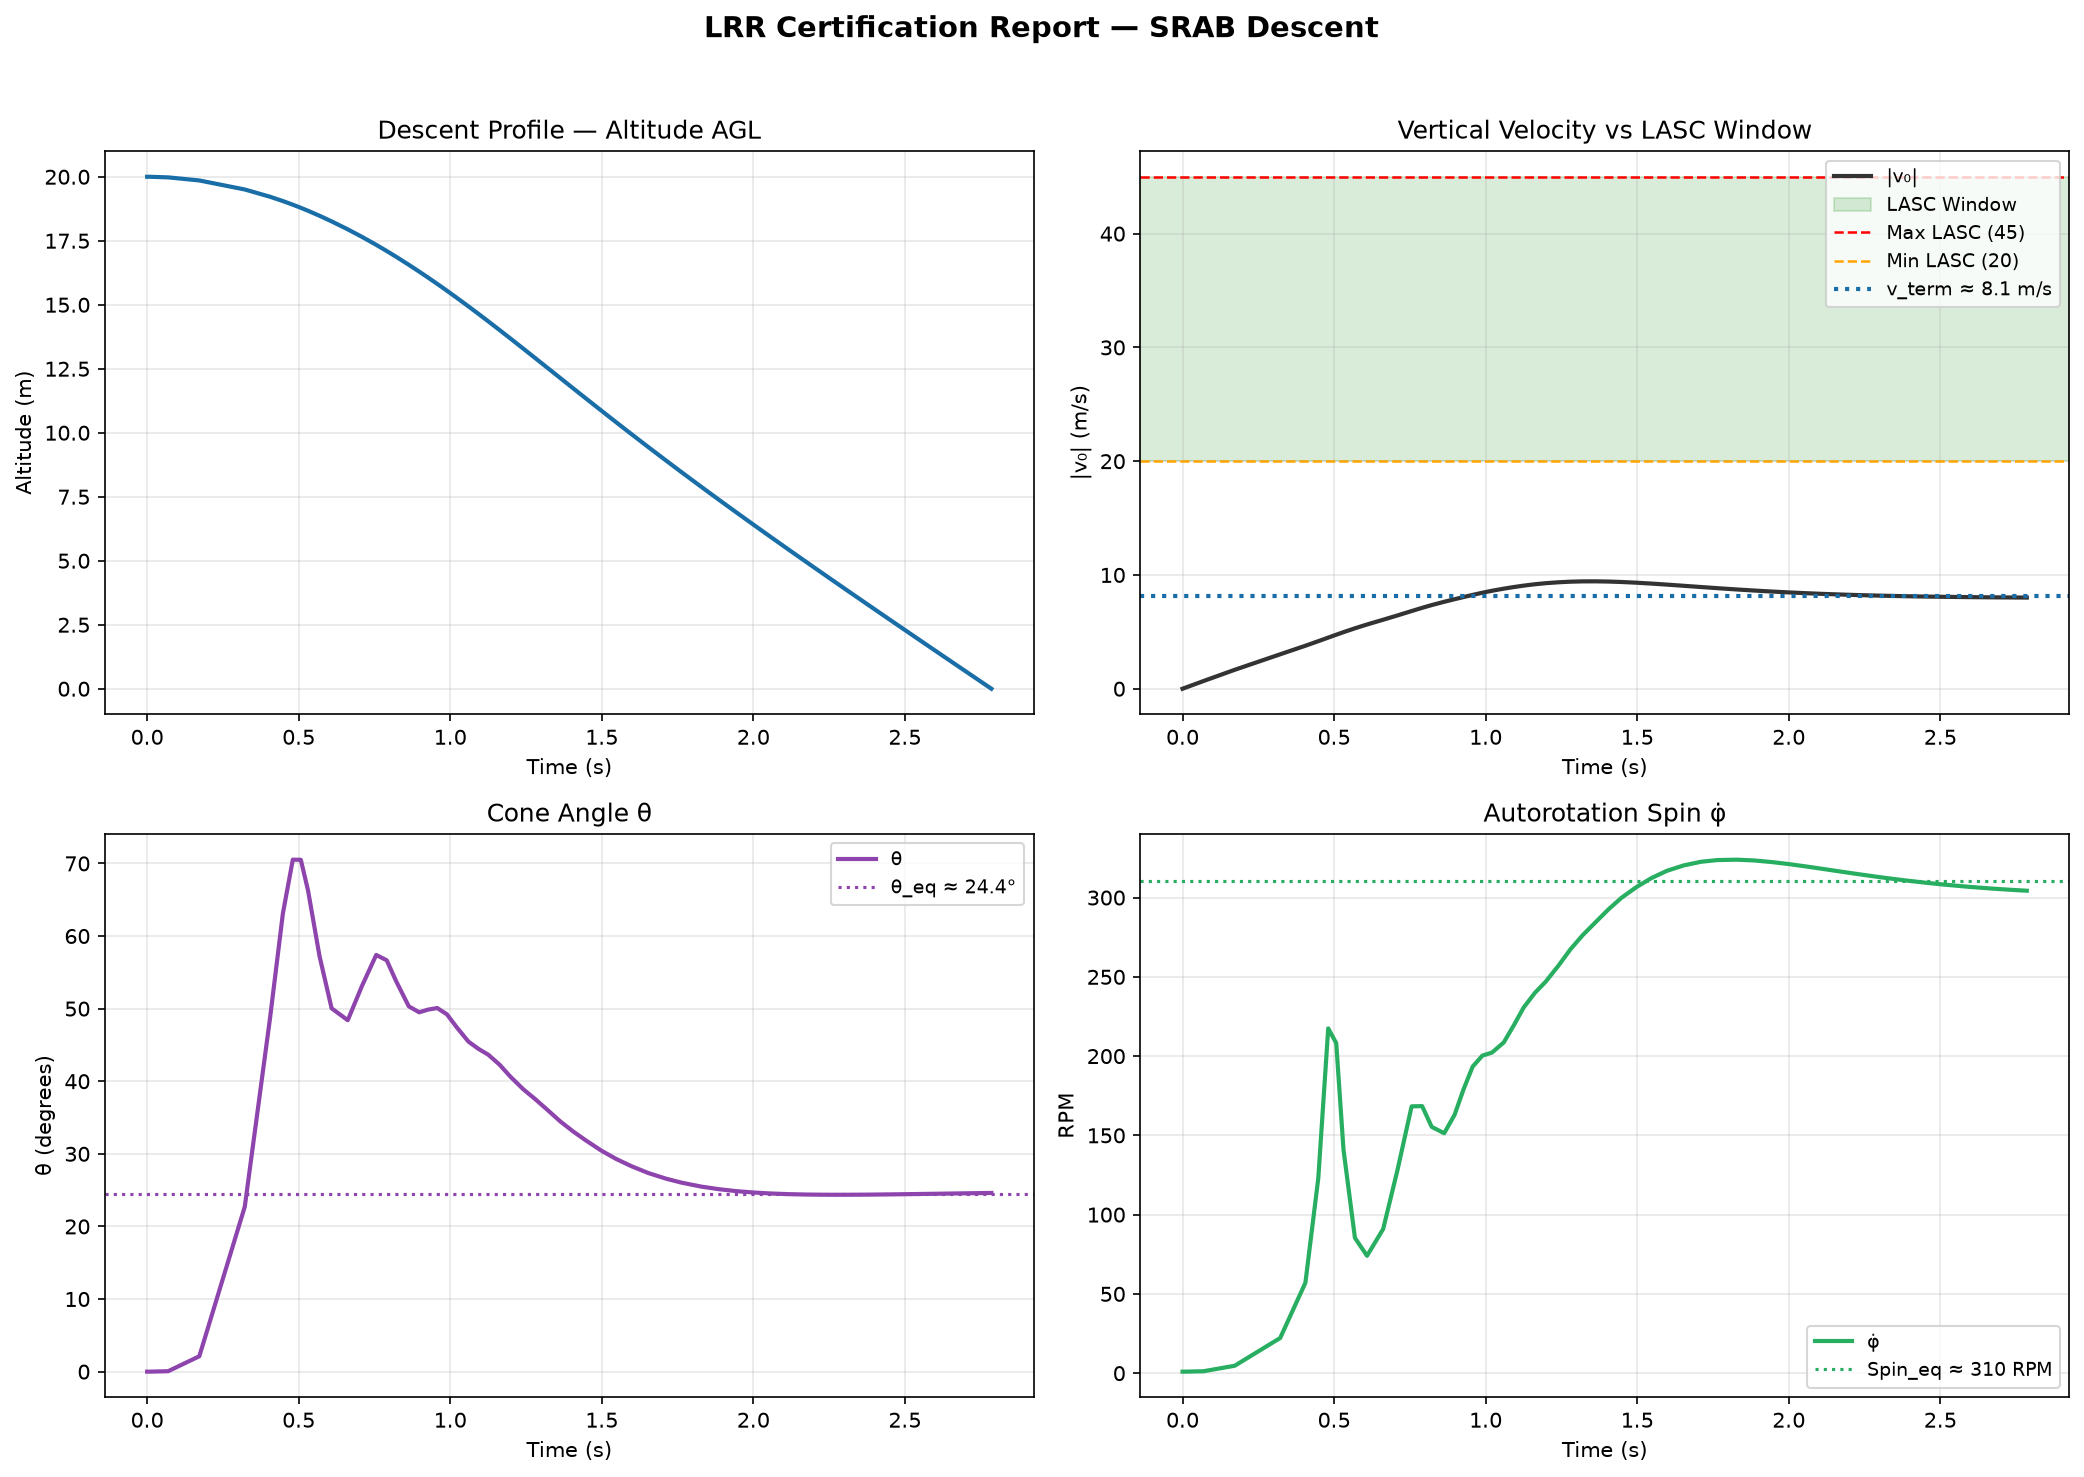
\includegraphics[width=0.9\textwidth]{figures/fig_test2_lrr.png}
\caption{LRR certification dashboard of Test~2 (Asa2, 4 wings, drone
drop from $\sim$20~m): the increased wing area (122.28~cm$^2$)
delivers a lower terminal velocity with a stable autorotation
state. The alpha-version onboard electronics were validated in this
drop, and the data confirmed the need for higher drop altitudes to
escape the transient regime.}
\label{fig:test2-lrr}
\end{figure}

Test~1 (Asa1, 4 wings) was the first time the samara autorotation
principle was observed in flight on the Helike project: the
prototype reached a stable coning motion within a fraction of a
second of release and the spin axis remained steady through the
descent, confirming that the deploy mechanism was passive and
deterministic. Test~2 (Asa2, 4 wings, wing area 122.28~cm$^2$)
increased the wing area by 12\% over Asa1 and was evaluated as the
intermediate candidate, reaching 8.04~m/s at impact with a stable
autorotation state; the same flight also carried the first
alpha-version onboard electronics, which recorded the rotation
profile with the flight IMU and produced the ENMC consolidated
dataset. The drone-altitude drops (Tests~1--2, $\sim$20~m) are too
short to reach the terminal velocity: the vehicle is still
accelerating at impact, so the measured values are transient and
must be compared against the simulated terminal values, not
directly against the LASC limit. The data from Tests~1--2 made it
clear that higher drop altitudes were required to leave the
transient regime, and Test~3 (Asa3, 4 wings, $\sim$30~m drone
drop, $\sim$200~g payload representative of the final assembly,
electronics onboard) was designed for exactly that --- the higher
release altitude and the realistic mass moved the impact point
closer to the steady autorotation regime. The same flight also
validated the onboard electronics, with the SRAB instrumented to
record rotation with the flight IMU (ENMC consolidated data).

\subsubsection{Geometry Comparison and Final Choice}

A comparative simulation of Asa2 (4 wings) vs. Asa3 (2 wings) showed
8.04 vs. 13.33~m/s terminal velocity after the radius optimization.
The Asa3 2-wing configuration (optimized aerodynamic radius
79.7~mm) was chosen as the final configuration for the mission: it
reaches the 20/1.5~m/s design target with a 1.5 safety factor on the
LASC 20~m/s limit, while offering lower mass and complexity than the
4-wing versions.

The choice between four and two wings is a direct trade-off between
redundancy and simplicity. The 4-wing variants (Asa1, Asa2) provide
geometric redundancy --- a single lost wing degrades performance
without preventing autorotation --- and a lower terminal velocity,
which increases the margin against the 20~m/s limit. However, they pay
for this in mass, rotating inertia and mechanical
complexity: each additional wing adds 3D-printed material, bonding
area and a potential failure surface, and the higher rotating mass
stores more kinetic energy at impact for the same descent velocity.
The 2-wing Asa3 exploits the same autorotation physics with roughly
half the wing area (58.7~cm$^2$ vs. 122.28~cm$^2$) and, being
lighter, spins faster at equilibrium (477~rpm vs. 372~rpm for the
4-wing test geometry), which increases the gyroscopic stiffness that
stabilizes the coning motion. At the cost of reduced geometric
redundancy, it still sits 1.5$\times$ below the regulatory limit, and
the drop-test evidence (Tests 1--3) confirms that deployment and
steady autorotation are deterministic with the passive geometry ---
there are no hinges or actuators to jam, so the redundancy argument
that motivates four wings is largely addressed by the mechanism's
inherent robustness rather than by part count. The mission risk
assessment (Appendix B) treats single-wing loss as a degraded-mode
event bounded by the same 20~m/s limit, and the mechanical
simplification of two wings directly supports the schedule-driven
development goal of the project.

% TODO: Test 4 (~200 m drop) is the next step for quantitative
% aerodynamic validation of the Asa3 2-wing configuration.
 % 4. Computational Simulation
\begin{enumerate}
\def\labelenumi{\arabic{enumi}.}
\setcounter{enumi}{4}
\item
  \textbf{Conclusions and Lessons Learned}
\end{enumerate}

\subsection{Conclusions}

The Helike \#213 mission demonstrates that a bioinspired autorotative
recovery system (SRAB) is a viable, simpler and more robust
alternative to conventional parachutes for 1P PocketQubes:

\begin{itemize}
\item The SRAB achieves the LASC regulatory impact velocity with a
  fully passive mechanism — no actuators, no pyrotechnics, no
  software dependency.
\item The computational model (4th-order rigid body + BEM + LEV
  correction) reproduces the measured drop-test behavior with
  sufficient fidelity for design decisions, and the full flight
  simulation (Dédalo launch vehicle + SRAB descent) certifies the
  recovery under real GFS conditions.
\item Compared with a conventional parachute, the SRAB reduces
  descent time by 36\% and total drift by 36\%, improving recovery
  accuracy at the cost of a higher — yet compliant — impact energy.
\item The three-filter review (SCSM compliance, Murphy analysis,
  timeline discipline) proved to be an effective engineering
  framework: it caught the non-parachute notification requirement
  (REC 10.2.1), drove the redundancy decisions in firmware and
  hardware, and kept the project aligned with the competition
  deadlines.
\end{itemize}

\subsection{Lessons Learned}

\begin{itemize}
\item \textbf{LASC 2025: optimization without redundancy is a trap.}
  Every subsystem of Helike has a backup path: SD + LittleFS, LoRa +
  local storage, hardware watchdog, passive recovery that does not
  depend on electronics.
\item \textbf{The parachute is the weakest link.} Replacing it with a
  passive aerodynamic mechanism removes the most failure-prone
  element of the recovery chain.
\item \textbf{Iterative drop testing beats simulation alone.} Each
  test cycle (Asa1 $\rightarrow$ Asa2 $\rightarrow$ Asa3) produced a
  measurable improvement in the model and in the design; the
  simulation-validated iteration loop is the core of the project
  methodology.
\item \textbf{Compliance is a design input, not a formality.} The
  SCSM requirements (kill switches, RBF, autonomy, notification)
  shaped the hardware schematic and the firmware FSM from day one.
\item \textbf{Team management:} the three-filter reviews force
  data-driven decisions with evidence artifacts (videos, logs, bench
  tests), which accelerates the transfer of knowledge from senior
  members to new members — every filter review is a training
  opportunity for the next generation of the team.
\end{itemize}
   % 5. Conclusions and Lessons Learned
\begin{enumerate}
\def\labelenumi{\arabic{enumi}.}
\setcounter{enumi}{5}
\item
  \textbf{References}
\end{enumerate}

% LASC / SCSM
[1] Latin American Space Challenge (LASC), ``Satellite Challenge
Standards Manual,'' Edition 7, Revision 1 (SCSM E07 R01), 2025.
Available at \url{https://lasc.space/}.

% Samara / LEV / autorotation literature
[2] U. M. Norberg, ``Structure, form, and function of flight in
engineering and the living world,'' \emph{Journal of Morphology},
vol. 252, no. 1, pp. 52--81, 2002.

[3] D. Lentink et al., ``Leading-Edge Vortices Elevate Lift of
Autorotating Plant Seeds,'' \emph{Science}, vol. 324, no. 5933,
pp. 1438--1440, 2009.

[4] C. J. Pennycuick, \emph{Modelling the Flying Bird}. Amsterdam,
The Netherlands: Academic Press, 2008.

% Autorotative descent / samara dynamics
[5] K. Yasuda, T. Azuma, ``The autorotation boundary in the flight of
samaras,'' \emph{Journal of Theoretical Biology}, vol. 185, no. 3,
pp. 313--320, 1997.

% PocketQube / CubeSat recovery
[6] R. McConnell, D. Das, ``Advances in Small Satellite Recovery
Systems,'' \emph{Proceedings of the Small Satellite Conference},
Logan, UT, USA, 2023.

% RocketPy
[7] RocketPy, ``RocketPy: Six Degree-of-Freedom Rocket Flight
Simulation,'' open-source software, 2024. Available at
\url{https://github.com/RocketPy-Team/RocketPy}.

% ENMC (Congresso Nacional de Engenharia Mecanica) — SRAB paper
[8] Serra Rocketry, ``Estudo e Desenvolvimento de um Sistema de
Recuperação Autorrotativo Bioinspirado (SRAB) para PocketQubes,''
submitted to the Congresso Nacional de Engenharia Mecânica (ENMC),
2026.
    % 6. References

% --- Appendices ---
\section*{Hazard Analysis Appendix}

The following hazards were identified and mitigated by design and/or
process, covering personnel safety during integration, launch and
recovery operations. The complete hazard analysis is presented in
Table~\ref{tab:hazards}:

\vspace{0.3cm}

\begin{table}[htbp]
\centering
\small
\setlength{\tabcolsep}{6pt}
% \tabularx exige a largura total (\textwidth) e usa a coluna do tipo 'X' para autoajuste
\begin{tabularx}{\textwidth}{p{3.5cm} X X} 
\toprule
\textbf{Hazard ID \& Title} & \textbf{Design Mitigation} & \textbf{Process Mitigation} \\
\midrule

\textbf{Hazard 1} \newline Battery thermal runaway &
BMS with multiple protections covering overcharge, overdischarge, short-circuit, and overcurrent conditions. &
Cells cycle-tested before integration. Battery charged only with approved charger, monitored during pre-launch, and RBF pin cuts all energy during transport. \\
\addlinespace

\textbf{Hazard 2} \newline Stored energy during integration &
Two independent mechanical kill switches (SW1/SW2) wired in parallel (NC) on main power line. RBF pin (SW3) in series cuts all energy when inserted. &
Pre-integration verification procedure checks kill switch activation. RBF removed only after installation in the deployer. \\
\addlinespace

\textbf{Hazard 3} \newline Sharp edges of SRAB wings &
Final geometry features rounded leading edges. &
Team wears handling gloves during integration. Recovery team briefed on wing handling. \\
\addlinespace

\textbf{Hazard 4} \newline RF interference with other teams &
Dedicated packet protocol with team ID, a reserved 915~MHz channel, and local storage for full data backup. &
Coordinated frequency allocation during operations. \\
\addlinespace

\textbf{Hazard 5} \newline Uncontrolled descent &
Passive deployment with no actuators, two-wing configuration for predictable recovery, keeping nominal impact energy low (17.8~J). &
Validated through three iterative simulation-and-test campaigns. \\

\bottomrule
\end{tabularx}
\caption{Hazard analysis and mitigations.}
\label{tab:hazards}
\end{table}
   % Appendix: Hazard Analysis
\textbf{\hfill\break
}

\textbf{Risk Assessment Appendix}

The second Mission Report appendix shall contain a Risk Assessment. This
appendix shall summarize risk and reliability concepts associated with
the project. All identified failure modes which pose a risk to mission
success shall be recorded in a matrix, organized according to the
mission phases identified by CONOPS.
     % Appendix: Risk Assessment
\section*{Engineering Drawings}

This appendix contains the revision-controlled technical drawings and
optional supporting material for the Helike \#213 subsystems.

\subsection{Drawing List}

The revision-controlled drawing set is listed in
Table~\ref{tab:drawings}. The electrical schematic of the subsystem
is presented in Fig.~\ref{fig:schematic}, the mechanical frame in
Fig.~\ref{fig:alba-frame} and the SRAB assembly in
Fig.~\ref{fig:srab-assembly}:

\begin{table}[htbp]
\centering
\small
\setlength{\tabcolsep}{6pt}
\begin{tabular}{>{\raggedright\arraybackslash}p{6cm}}
\toprule
\textbf{Drawing / Document} \\
\midrule
Electrical schematic (KiCad, U1--U6, SW1--SW3) \\
1P Alba Orbital frame (aluminum + FRP backplate) \\
SRAB wing assembly (hub + 2 wings, PETG) \\
SRAB wing geometry — Asa1 contour (DXF) \\
SRAB wing geometry — Asa2 contour (DXF) \\
SRAB wing geometry — Asa3 contour (DXF) \\
PocketQube 1P mechanical structure \\
ESP32-C3 pinout \\
Integrated assembly \\
\bottomrule
\end{tabular}
\caption{Drawing list.}
\label{tab:drawings}

\end{table}

\begin{figure}[htbp]
\centering
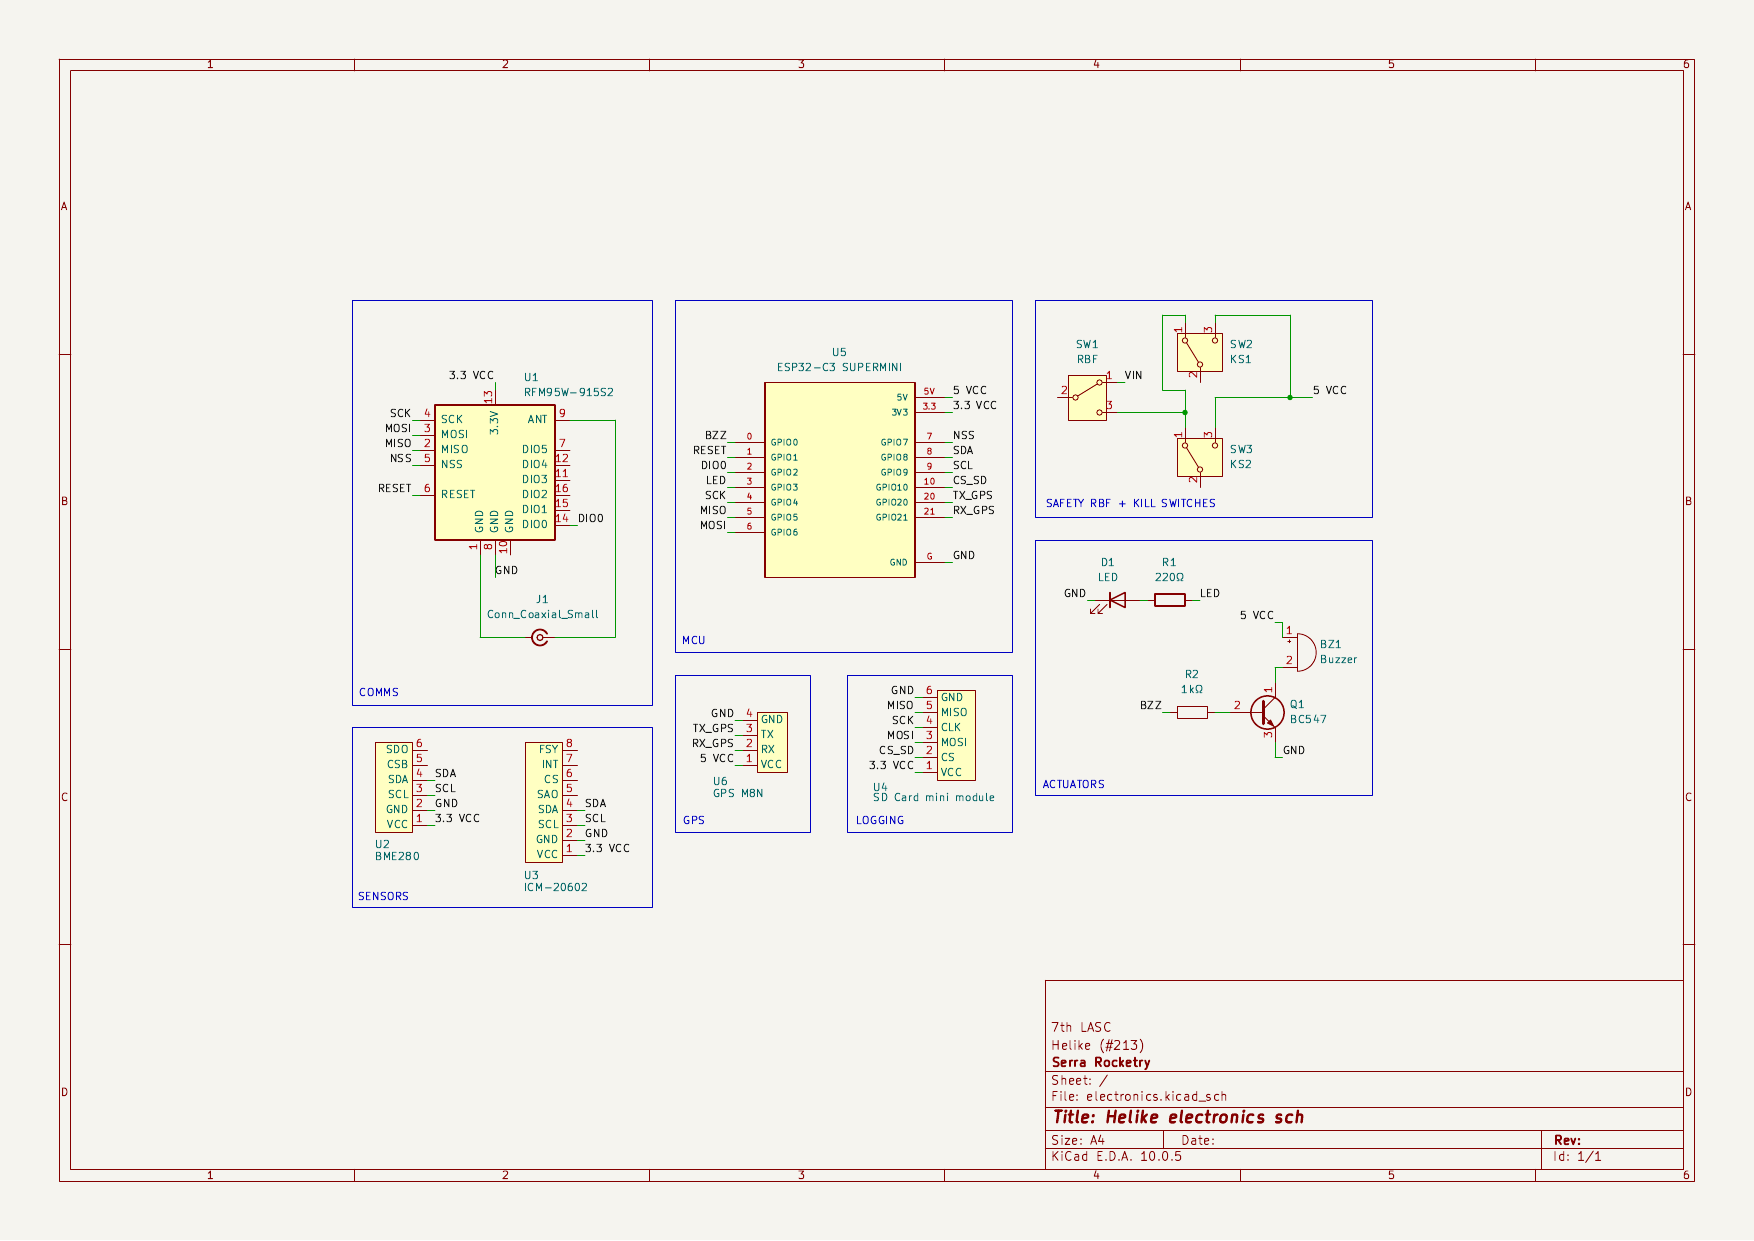
\includegraphics[width=0.9\textwidth]{figures/fig_schematic.png}
\caption{Electrical schematic of Helike \#213 (KiCad). U1: ESP32-C3
Super Mini; U2: LoRa RFM95W-915S2; U3: BME280; U4: ICM-20602; U5: GPS
NEO-8M; U6: SD card module; SW1/SW2: kill switches (Z axis); SW3: RBF
pin; J1: SMA antenna; D1/BZ1: status LED and buzzer.}
\label{fig:schematic}
\end{figure}

\begin{figure}[htbp]
\centering
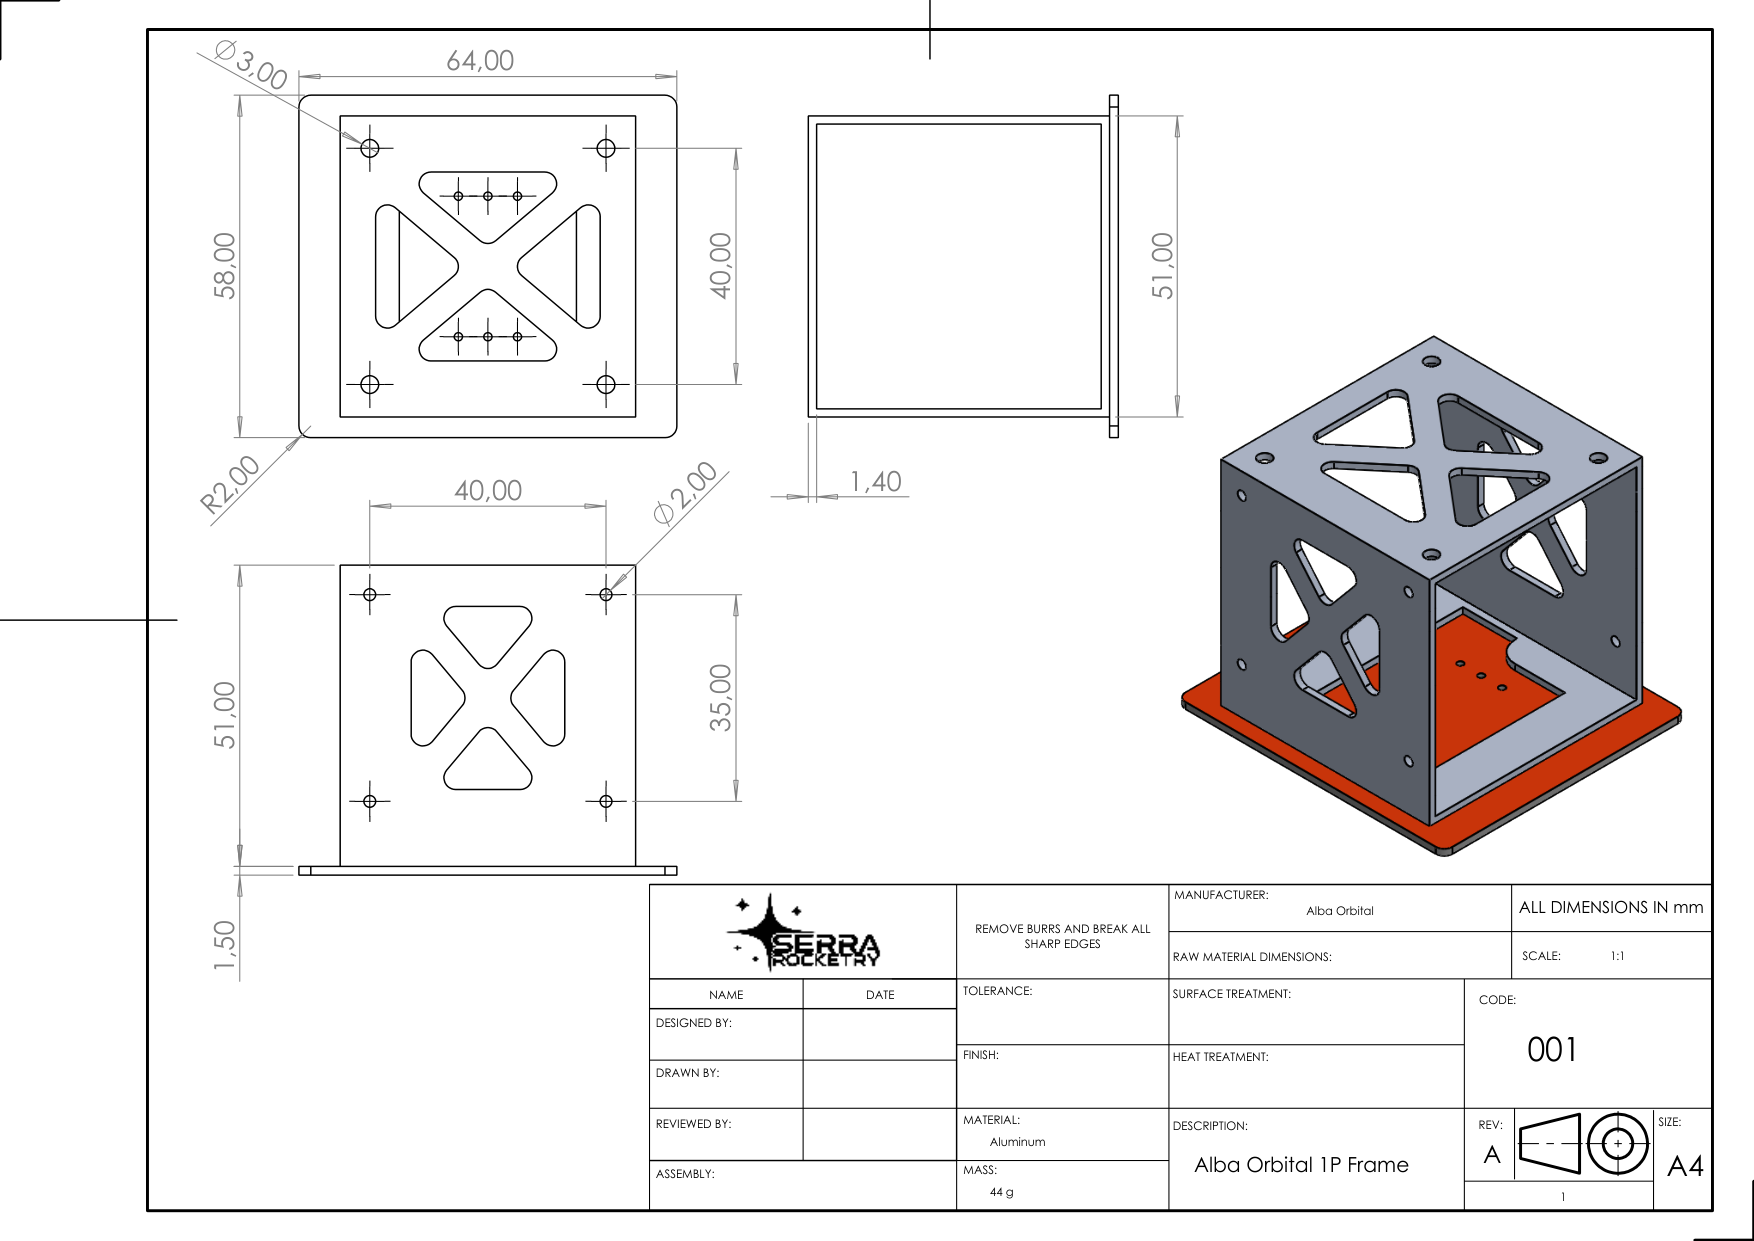
\includegraphics[width=0.8\textwidth]{figures/1P_ALBA_ORBITAL_frame_p1.png}
\caption{Technical drawing of the 1P Alba Orbital frame: 51$\times$51
mm aluminum structure with 1.4~mm wall thickness, 1.5~mm FRP
backplate and a total mass of 44~g.}
\label{fig:alba-frame}
\end{figure}

\begin{figure}[htbp]
\centering
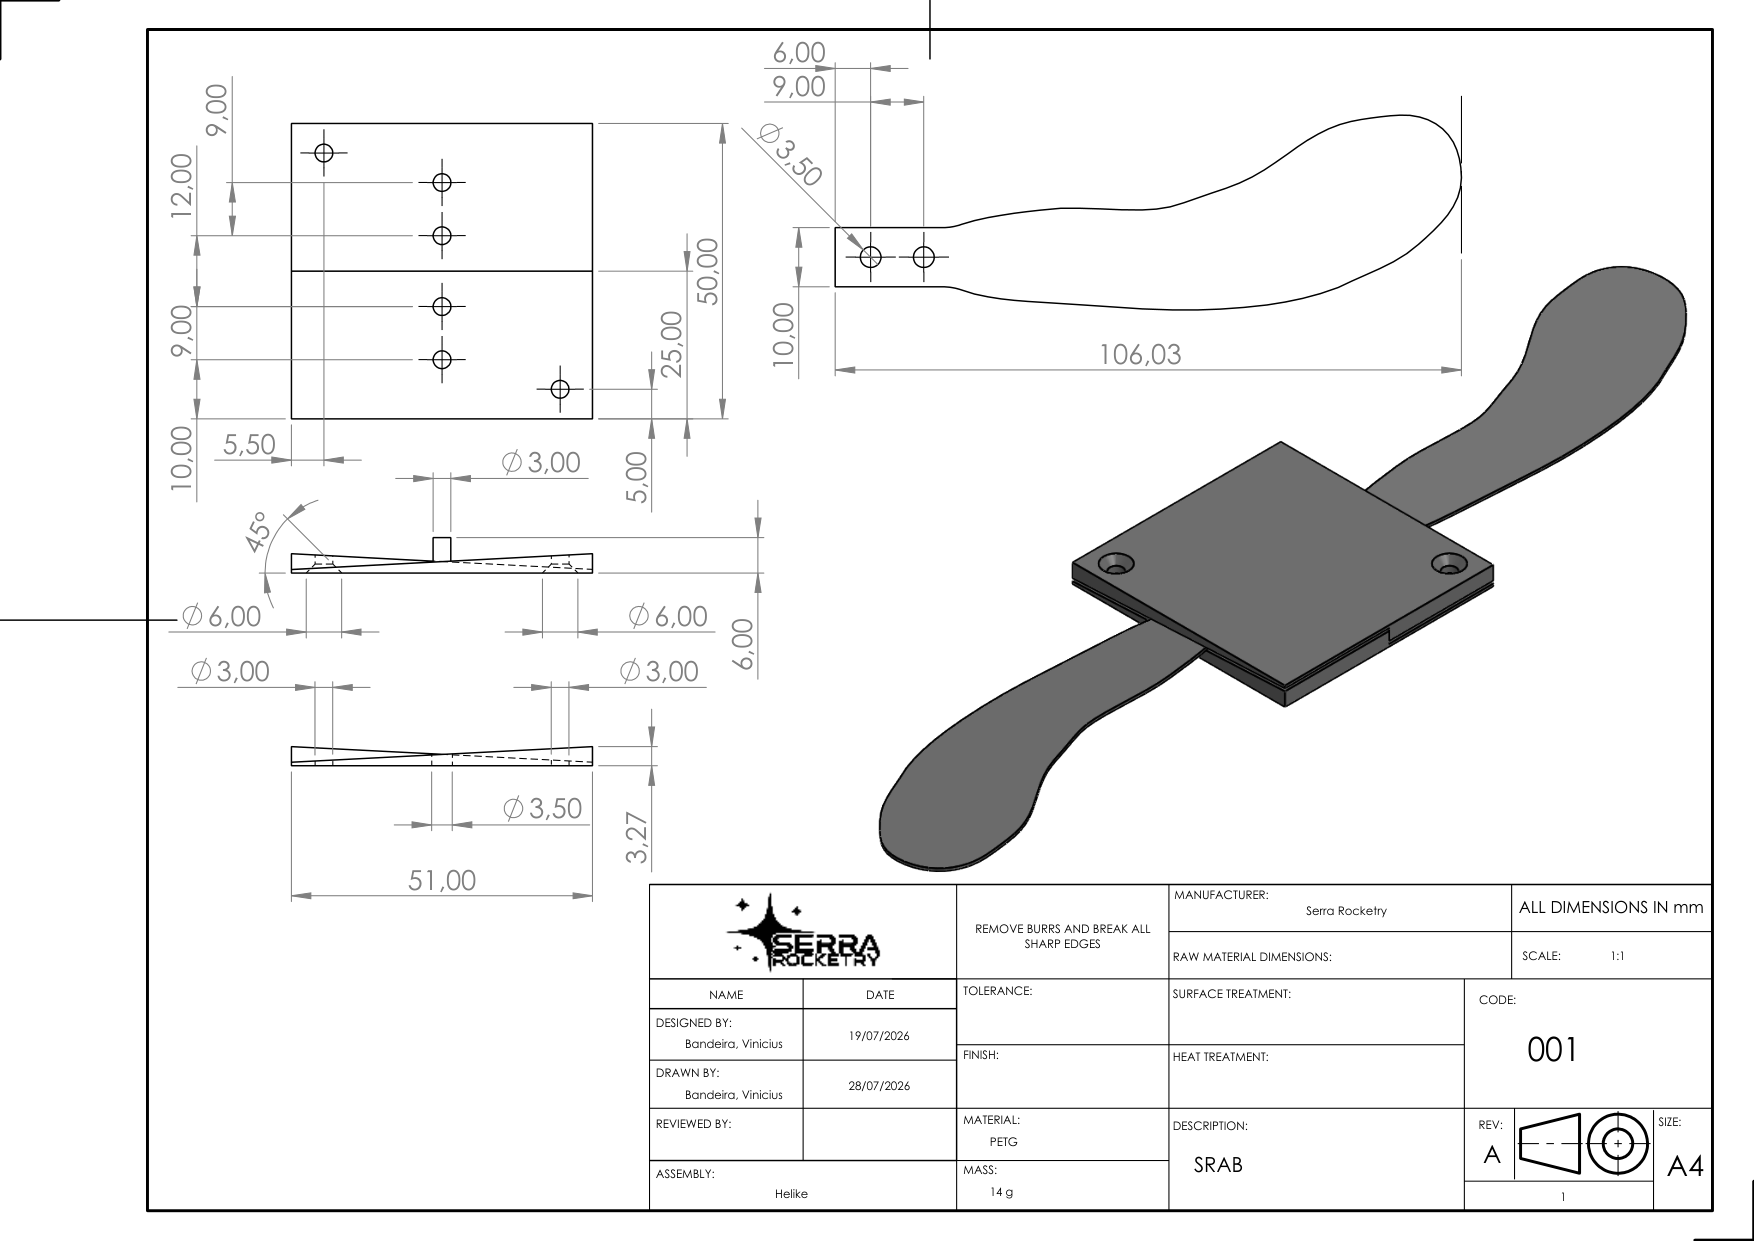
\includegraphics[width=0.8\textwidth]{figures/srab_only_assy_p1.png}
\caption{Technical drawing of the SRAB assembly: central 50$\times$50
mm hub and the two mirrored autorotative wings (PETG, total mass
14~g).}
\label{fig:srab-assembly}
\end{figure}

\begin{figure}[htbp]
\centering
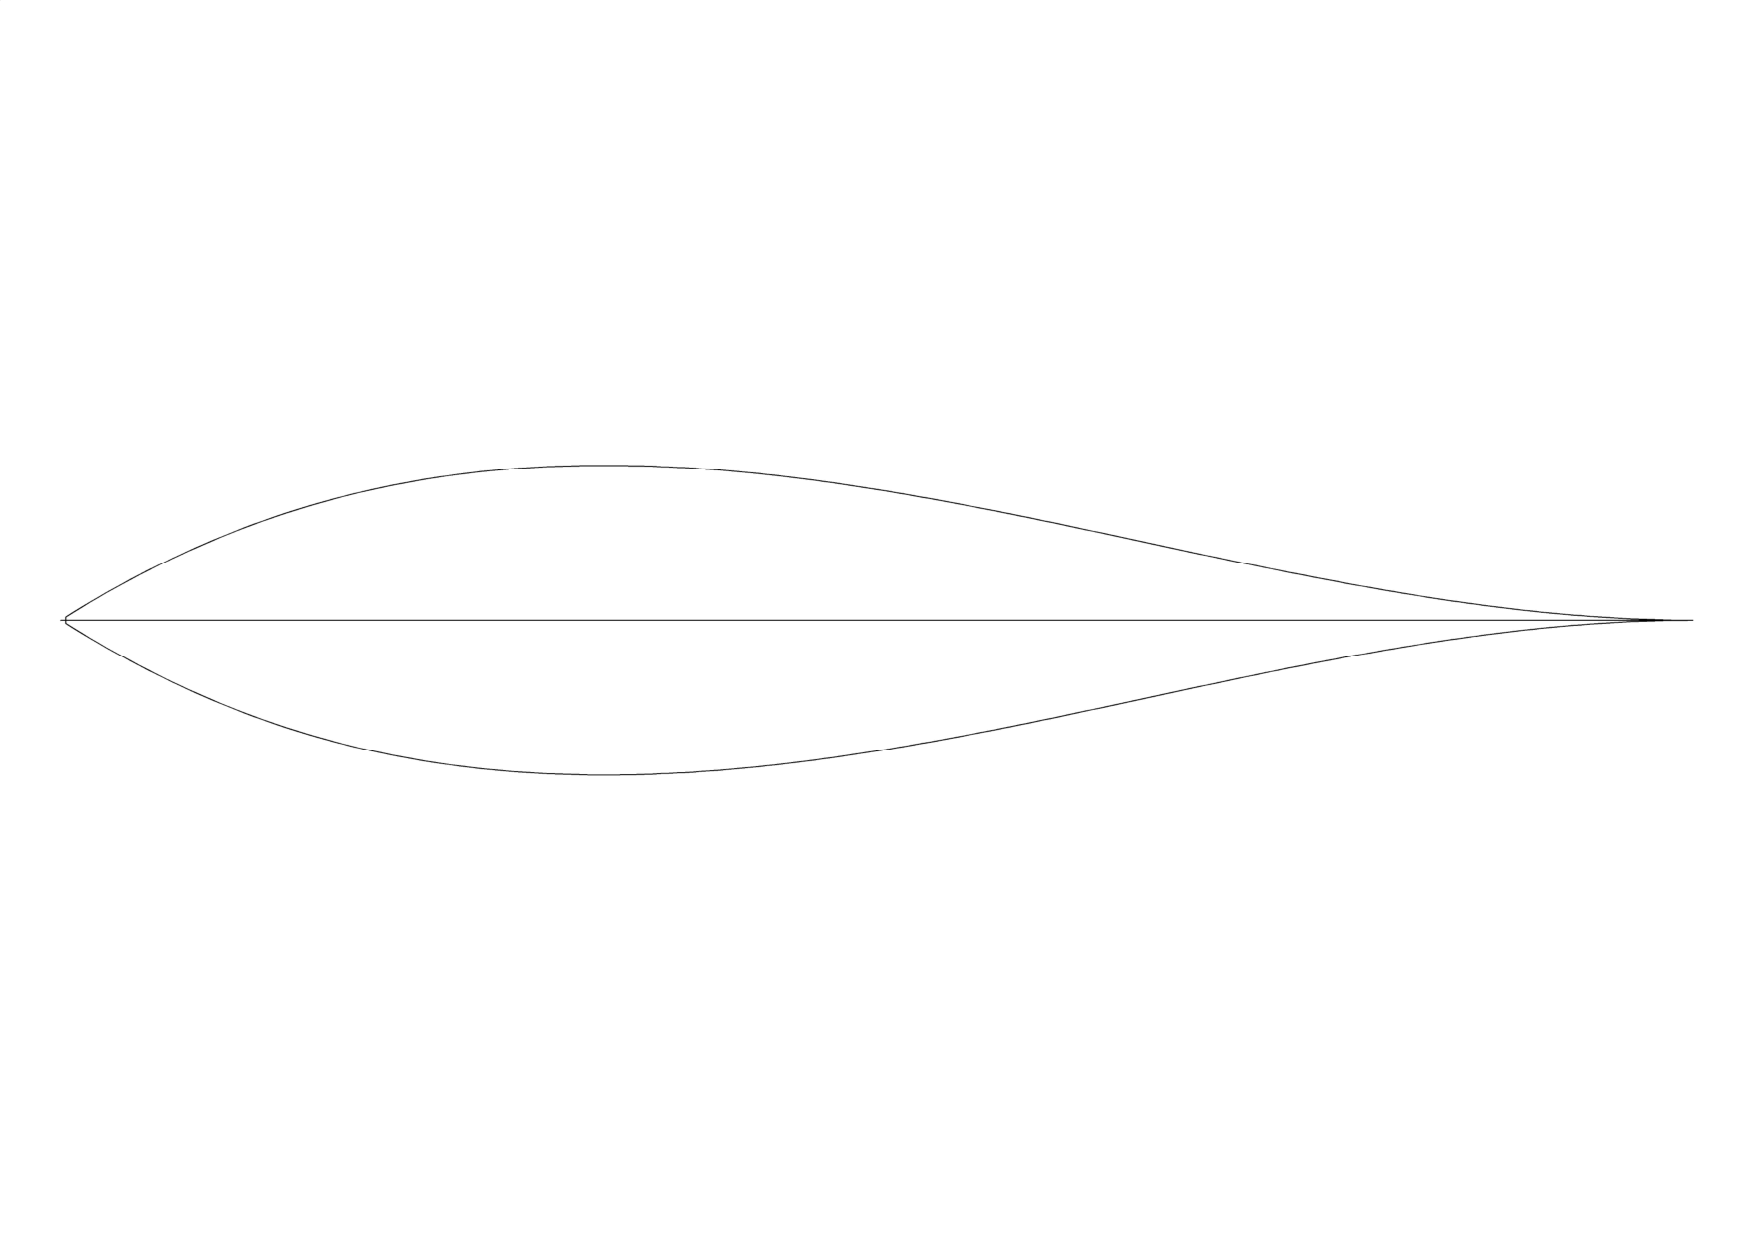
\includegraphics[width=0.9\textwidth]{figures/Asa1_dxf_p1.png}
\caption{2D contour drawing (DXF) of Asa1 wing geometry: 4-wing
configuration, base chord and tip dimensions marked. Used in the
first physical drop campaign (Test 1).}
\label{fig:asa1-dxf}
\end{figure}

\begin{figure}[htbp]
\centering
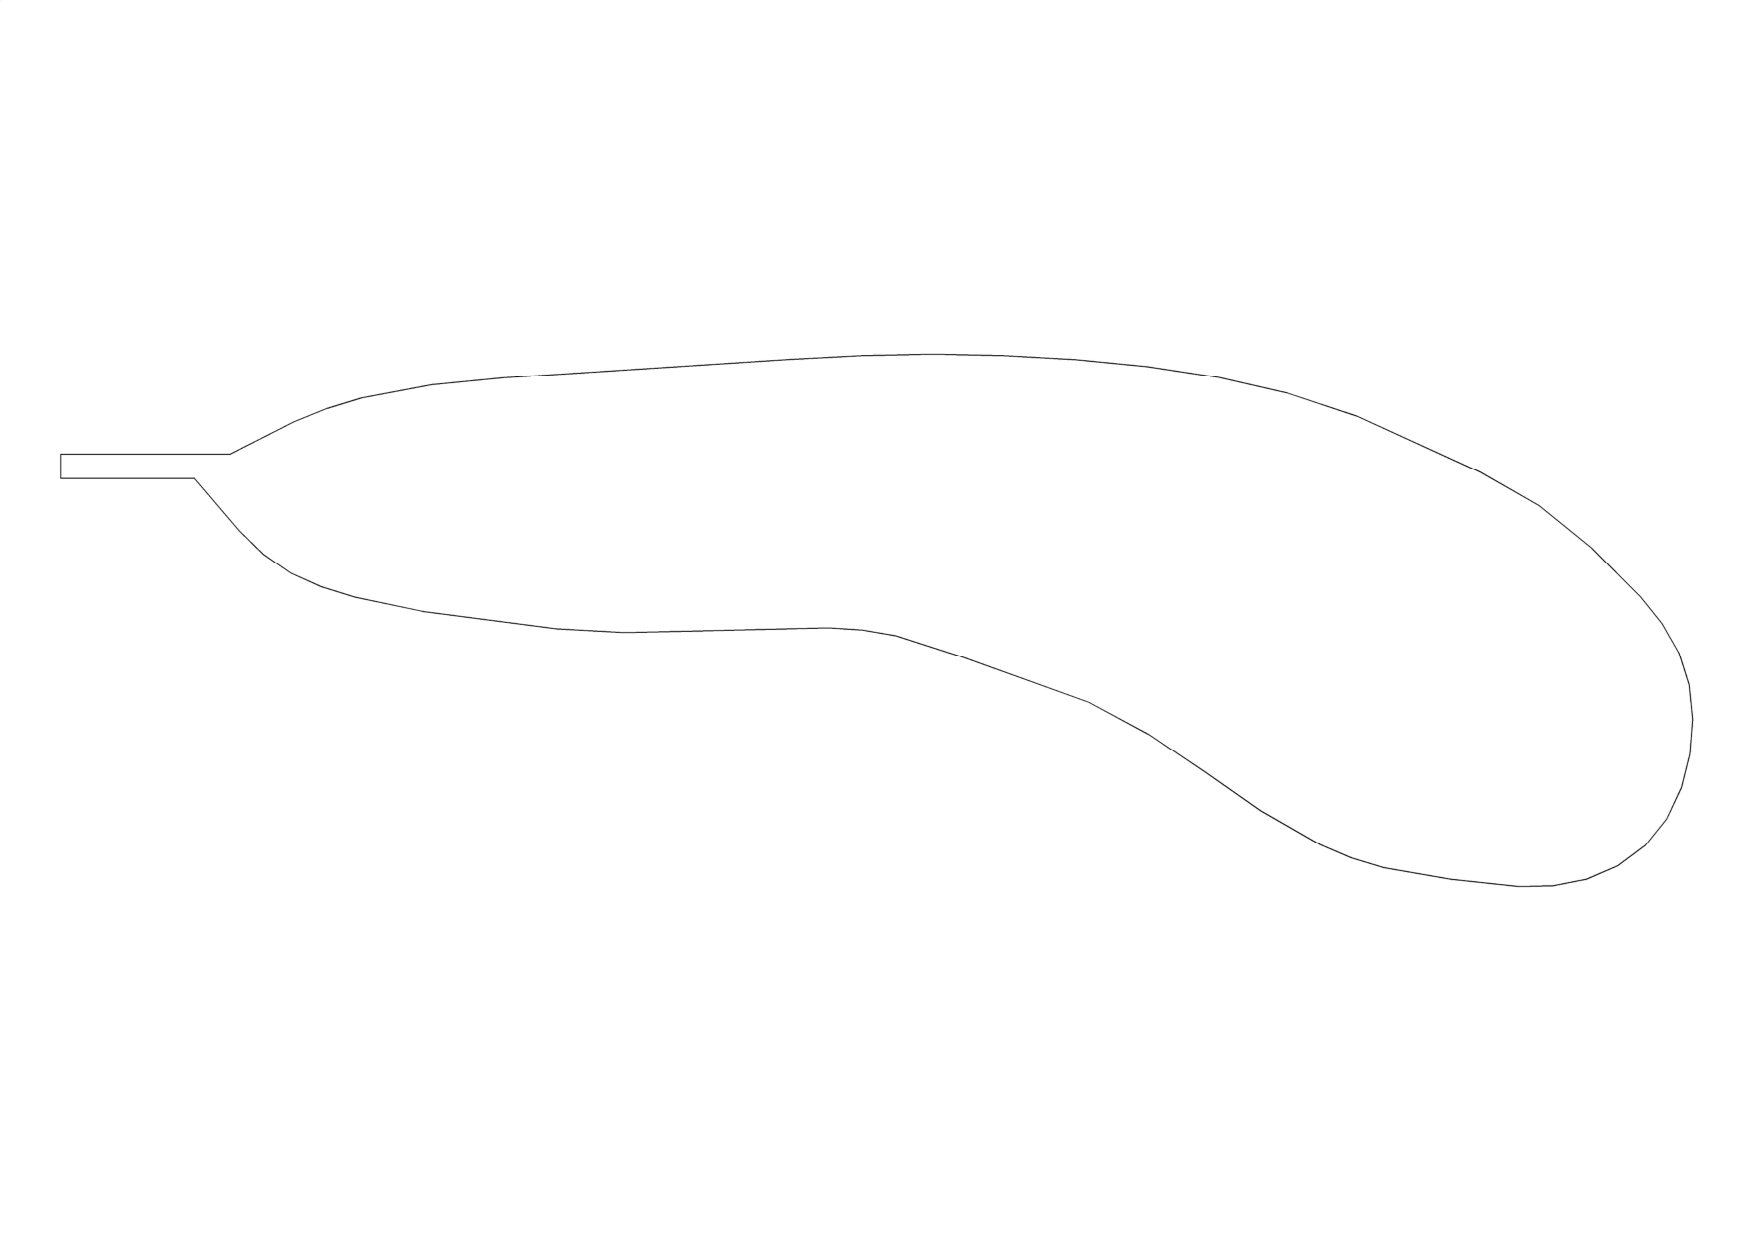
\includegraphics[width=0.9\textwidth]{figures/Asa2_dxf_p1.png}
\caption{2D contour drawing (DXF) of Asa2 wing geometry: 4-wing
configuration with increased area and realigned chord relative to
Asa1. Used in the second drop campaign (Test 2).}
\label{fig:asa2-dxf}
\end{figure}

\begin{figure}[htbp]
\centering
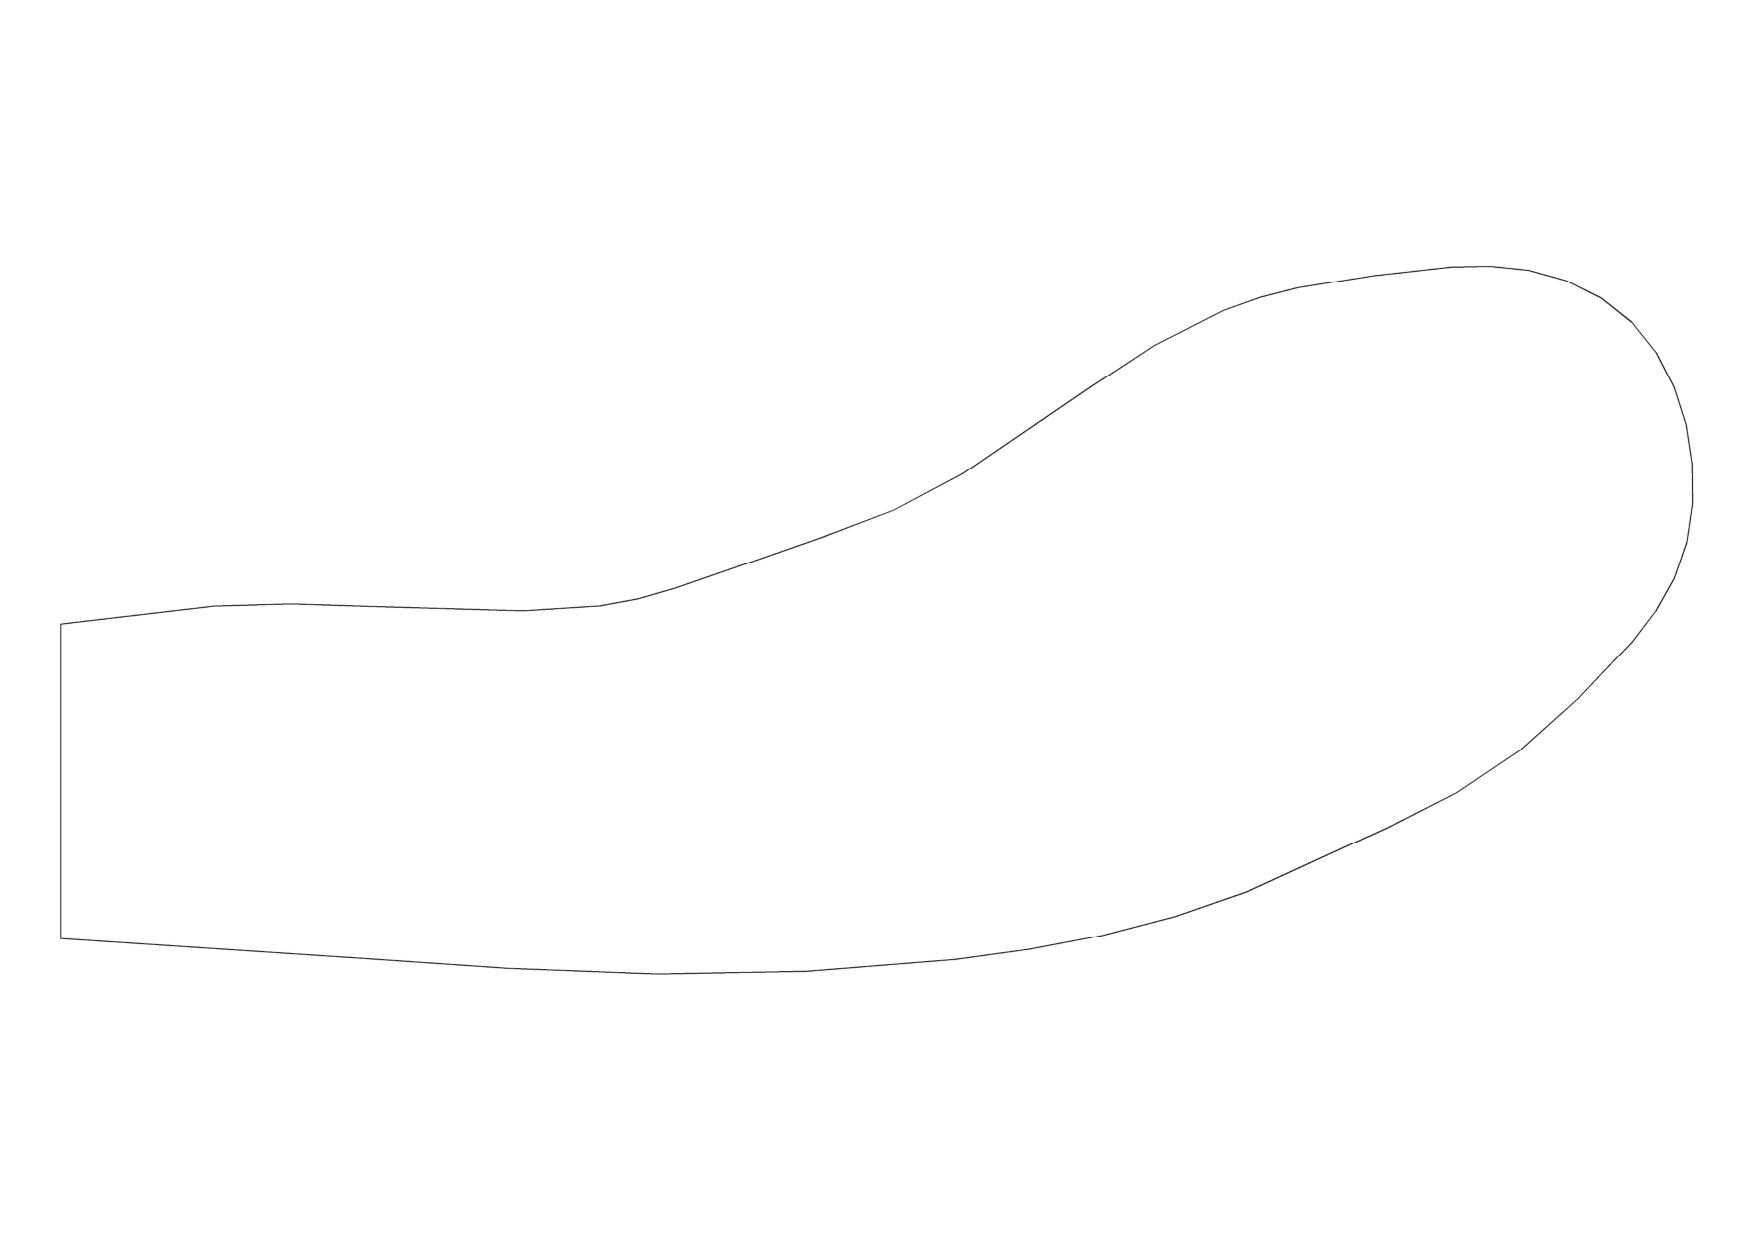
\includegraphics[width=0.9\textwidth]{figures/Asa3_dxf_p1.png}
\caption{2D contour drawing (DXF) of Asa3 wing geometry: 2-wing
mission-final configuration. Optimised radius 79.7~mm, chord and
pitch distribution for the target $V_F = 13.33$~m/s with FS 1.5.}
\label{fig:asa3-dxf}
\end{figure}

\subsection{Optional Appendices}

\subsubsection{SRAB Wing Geometry}

The wing geometries evolved through three design iterations, driven
by the simulation-to-field comparison loop described in Section 4:

\begin{itemize}
\item \textbf{Asa1} — 4 wings, first prototype: v$_{impact}$ =
  7.68~m/s, 306.8~rpm, 13.5$^{\circ}$.
\item \textbf{Asa2} — 4 wings, increased area and realignment:
  v$_{impact}$ = 8.04~m/s, 306.9~rpm, 24.4$^{\circ}$ — candidate
  configuration.
\item \textbf{Asa3} — 2 wings (mission final): reduced mass and
  complexity, $v \approx 13.33$~m/s terminal, within the LASC
  20~m/s limit with a 1.5 safety factor.
\end{itemize}

The 2D contour drawings (DXF) for each iteration are presented in
Fig.~\ref{fig:asa1-dxf}, Fig.~\ref{fig:asa2-dxf} and
Fig.~\ref{fig:asa3-dxf} above.

\subsubsection{Test Data}

% TODO: include CSV logs, telemetry plots, simulation-vs-field
% comparison plots, photos of Asa1/Asa2 prototypes and drop-test
% videos once the instrumentation campaign (Test 4, ~200 m) is
% complete.

\subsubsection{Computational Simulation}

The 4th-order autorotation model, calibrated parameters, simulation
scripts (RocketPy + SRAB extension) and the geometry heat-map are
maintained in the repository under \texttt{extras/wing-analysis/}.
The full-flight simulation (Dédalo + SRAB) is documented in the
notebook \texttt{01\_simulacao\_dedalo.ipynb}.
 % Appendix: Engineering Drawings and Optional

% --- Template guidance (NOT part of the final report) ---
% Instrucoes de formatacao do template LASC, preservadas para consulta:
%   sec-procedure.tex   (2. Procedure for submission)
%   sec-guidelines.tex  (3. General Guidelines and Required Elements)
%   sec-formatting.tex  (4. Detailed Formatting Instructions)

\end{document}
